\section{Comunicazione}\label{capitolo5}
La comunicazione tra processi è il cuore di tutti i sistemi distribuiti, infatti, non ha senso studiare i sistemi distribuiti senza esaminare come i processi su posti macchine diverse si scambiano le informazioni. La comunicazione nei sistemi distribuiti si basa sempre sullo scambio dei messaggi a basso livello come fornito dalla rete sottostante, anche se ciò rende la realizzazione del sistema distribuito molto complicata.\\
In questo capitolo analizzeremo prima di tutto le regole che i diversi processi devono rispettare per comunicare tra loro, queste regole sono conosciute anche come protocolli e solitamente vengono strutturati a livelli.\\
Analizzeremo in seguito tre modelli di comunicazione molto diffusi, le chiamate a procedure remote (RPC, \emph{remote procedure call}), i middleware orientati agli oggetti (MOM, \emph{message-oriented middleware}) e gli \emph{streaming} di dati. Ed infine analizzeremo il problema dell'invio di dati a destinatari multipli, ovvero, il \emph{multicast}.\\
\subsection{Il modello OSI}
A causa della mancanza di una memoria condivisa tutta la comunicazione nei sistemi distribuiti avviene mediante tramite l'invio e la ricezione di messaggi a basso livello. Quando un processo \emph{A} vuole comunicare con un processo $B$ prima di tutto costruisce un messaggio nel proprio spazio degli indirizzi e poi effettua una \emph{chiamata di sistema} che fa in modo che il SO si occupi dell'invio del messaggio attraverso la rete fino a raggiungere $B$. Anche se il principio è semplice esistono diversi ostacoli al completamente di questa operazione, prima di tutto $A$ e $B$ devono concordare sul significato dei bit inviati, esistono molti altri aspetti sui quali bisogna accordarsi, come il valore in volt usati per indicare un bit a 1, individuare l'ultimo bit del messaggio, bisogna inoltre capire se un messaggio è stato danneggiato o perso ecc.\\
Per poter trattare facilmente i numerosi aspetti di una comunicazione la \emph{international standard organization} (ISO) ha sviluppato un modello di riferimento che identifica i vari livelli di comunicazione coinvolti, gli assegna dei nomi standard e identifica le diverse funzionalità per ogni livello. Questo modello è chiamato \textbf{open system interconnection reference model} o più comunemente modello \textbf{ISO OSI} ed è illustrato in \figurename\,\ref{img:osi}
\begin{figure}[htb]
\centering
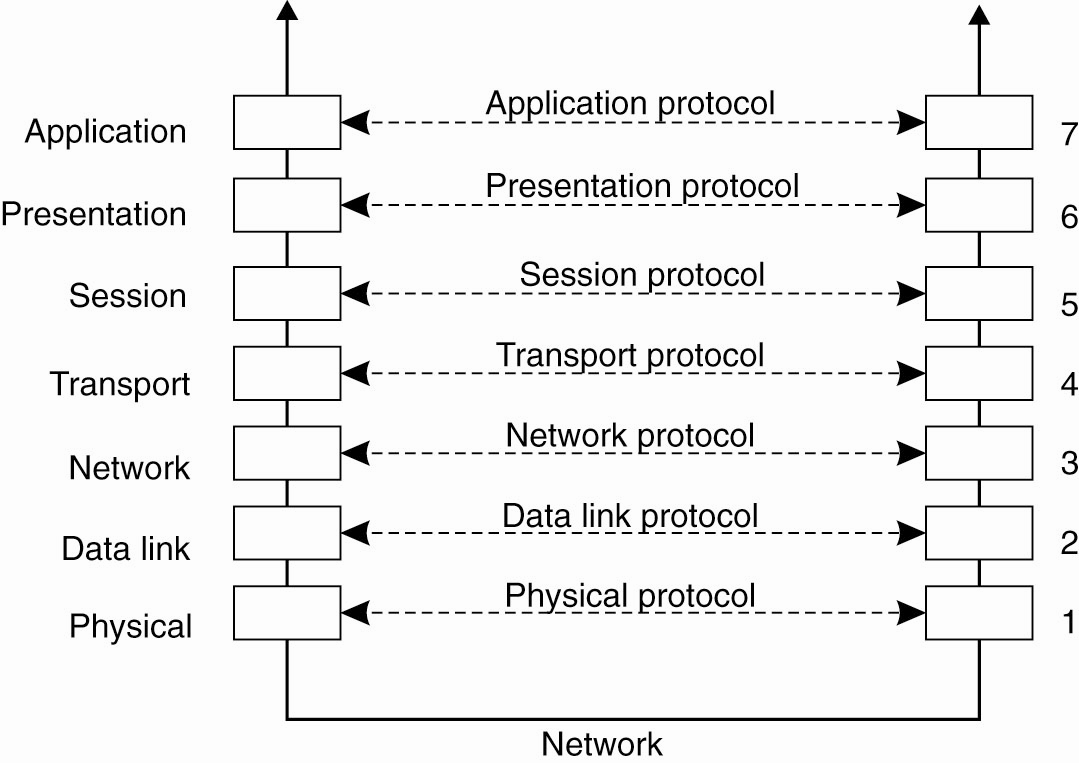
\includegraphics[scale=0.4]{img/osi.png}
\caption{Modello ISO OSI}\label{img:osi}
\end{figure}
Tuttavia è bene far presente che i protocolli sviluppati nel modello OSI non sono stati mai ampiamente utilizzati, tuttavia il modello sottostante si è rivelato particolarmente utile per comprendere le reti di computer.\\
Il modello OSI è progettato per consentire la comunicazione tra sistema aperti ovvero tra sistemi preparati per comunicare tramite regole standard che ne regolano il formato, i contenuti ed il significato di messaggi ricevuti ed inviati. Queste regole sono dette \textbf{protocolli} e devono essere concordate a priori per permettere la comunicazione tra gruppi di computer.\\
Esistono due grandi tipologie di protocolli, quelli \textbf{orientati alla connessione} nei quali mittente e destinatario stabiliscono esplicitamente una connessione prima di scambiarsi dei dati ed alla fine devono rilasciare tale connessione.
Con i protocolli \textbf{senza connessione} non è necessaria alcuna premessa, quando il messaggio è pronto il mittente invia il messaggio come nel caso di un invio di una lettera.\\
Nel modello OSI la comunicazione è suddivisa in sette livelli o \emph{layer}, ogni livello tratta uno specifico aspetto della comunicazione, in modo da suddividere il problema in parti gestibili ciascuna delle quali può essere trattata indipendentemente. Per realizzare questo meccanismo ogni livello fornisce un'interfaccia al livello superiore, la quale specifica un insieme di operazioni che il livello è pronto a fornire.\\
Quando un processo $A$ sulla macchina 1 vuole comunicare con un processo $B$ sulla macchina 2 costruisce un messaggio e lo passa al livello applicativo sulla sua macchina; tale livello potrebbe essere una procedura ad una libreria oppure implementato in qualche altro modo come ad esempio all'interno del sistema operativo. Il software a livello applicativo aggiunge un intestazione (\emph{header}) all'inizio del messaggio e passa tutto al livello di presentazione tramite l'interfaccia tra i livelli 6 e 7. A sua volta il livello di presentazione passa il messaggio al livello di sessione non prima di aver aggiunto il suo \emph{header} e così via. Alcuni livelli aggiungono oltre all'header anche un \emph{trailer} in chiusura al pacchetto come mostrato in \figurename\,\ref{img:header}.
\begin{figure}[htb]
\centering
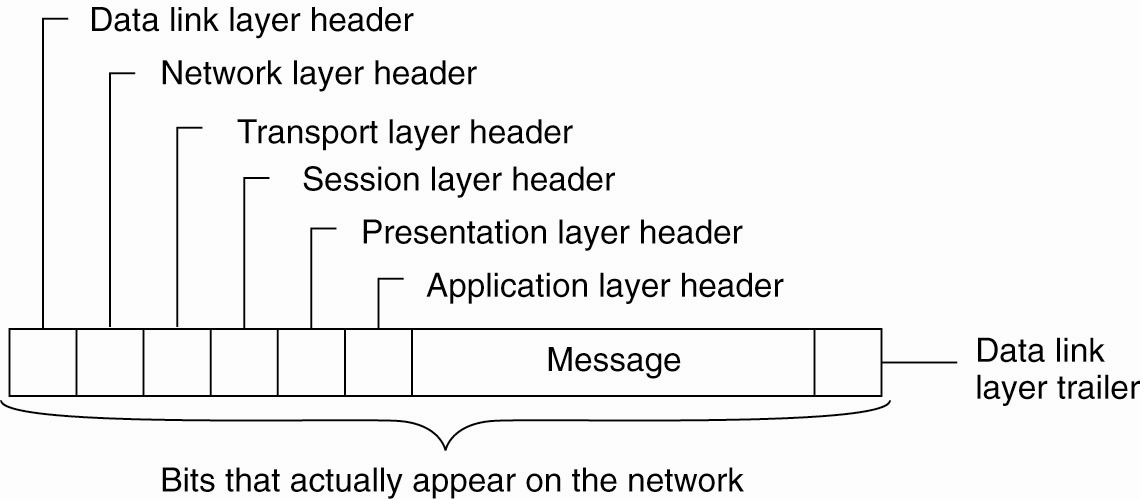
\includegraphics[scale=0.4]{img/header.png}
\caption{Elenco header e trailer di un messaggio che attraversa i vari layer}\label{img:header}
\end{figure}
Quando il messaggio raggiunge il fondo esso viene trasmesso dal livello fisico sul mezzo di trasmissione. Quando il messaggio raggiunge la macchina 2 viene passato verso l'alto e ogni livello stacca la sua intestazione e la esamina, infine il messaggio raggiunge il suo destinatario , ovvero il processo B il quale può rispondere utilizzando il percorso inverso.\\
Ogni livello ha il suo protocollo che può essere cambiato indipendentemente dagli altri ed è proprio questa indipendenza a rendere i protocolli a livelli interessanti.\\
L'insieme di protocolli usati in un particolare sistema è detto \textbf{suite di protocolli} o \textbf{stack di protocolli}.
\subsubsection{I layer}
Analizziamo ora i diversi layer che compongono il modello OSI, vedremo quali sono le loro funzionalità e dove possibile indicheremo quali protocolli sono attualmente utilizzati nell'ambito di internet.
Partiamo dai tre livelli più bassi della suite di protocolli, insieme questi tre livelli implementano le funzioni base di una rete di computer.\\
Il \emph{livello fisico} trasmette gli 0 e gli 1 sul canale fisico di comunicazione, elementi importanti per questo livello sono la quantità di volt che contraddistingue gli 0 e gli 1, il numero di bit al secondo, la possibilità di trasmettere in entrambe le direzioni, infine rivestono una notevole importanza la forma dei connettori (\emph{plug}) ed il numero di piedini (\emph{pin}). Il protocollo che identifica questo livello ha a che fare con la standardizzazione delle interfacce elettriche e meccaniche e di segnale; un esempio di questi standard è l'interfaccia RS-232-C per la comunicazione seriale.\\
Il livello \emph{data link} si occupa della rilevazione e della correzione degli errori di trasmissione. Per fare ciò il data link layer raggruppa i bit in unità chiamate \textbf{frame} e controlla che ogni frame sia ricevuto correttamente. Per eseguire questo compito il livello di collegamento dei dati applica un \emph{pattern} di bit all'inizio ed alla fine di ogni frame per delimitarli ed eseguire una \textbf{somma di controllo} (\emph{checksum}) sommando tramite algoritmi specifici i byte del frame ed inserisce tale somma nei campi all'inizio o alla fine del frame.
All'arrivo di un nuovo pacchetto il livello data link esegue la somma sui dati arrivati e la confronta con quella inviata insieme al pacchetto nel caso le due checksum coincidano il pacchetto è considerato corretto, in caso contrario il destinatario ne richiede la ritrasmissione grazie al numero di sequenza inserito nell'header del data link.\\
Il \emph{livello di rete} si occupa del \textbf{routing} dei pacchetti, ovvero, della scelta del percorso ottimale che permetta ad un pacchetto di andare da un mittente ad un destinatario.
Il problema si complica in quanto il percorso più breve non è sempre quello ottimo. Al momento il protocollo di rete più utilizzato è l'IP (\textbf{Internet Protocol}) senza connessione che è parte dei protocolli Internet. Un \textbf{pacchetto} IP può essere inviato senza alcun preparativo. Ogni pacchetto è instradato verso la sua destinazione indipendentemente da tutti gli altri.\\
Il \emph{livello di trasporto} costituisce l'ultima parte di quelli che possiamo definire \emph{stack del protocollo di rete di base} nel senso che implementa tutti i quei servizi non forniti dall'interfaccia del livello di rete ma necessari per l'implementazione di applicazioni di rete. In altre parole il livello di trasporto in un qualcosa di utilizzabile.\\
Uno dei compiti del livello di trasporto è quello di fornire una connessione affidabile anche se molte applicazioni gestiscono autonomamente la perdita di pacchetti.
Quando arriva un messaggio dal livello applicativo il livello di trasporto lo spezza in parti sufficientemente piccole per essere trasmesse ed assegna un numero di sequenza. Le informazioni nell'header del livello di trasporto riguardano il numero di pacchetti inviati, il numero di pacchetti ricevuti, quali devono essere ritrasmessi e così via.\\
Connessioni di trasporto affidabili possono essere costruite sopra servizi di rete orientati alla connessione o senza connessione. Nel primo caso i pacchetti arriveranno nella sequenza corretta, nel secondo caso non vi è alcun metodo per stabilire a priori l'ordine di arrivo dei pacchetti, ed è compito del software del livello di trasporto di riordinare i dati. Un aspetto importante del livello di trasporto è quello di fornire questo comportamento \emph{end-to-end}.\\
Il protocollo di trasporto di Internet è chiamato \textbf{TCP (transmission control protocol)}. La combinazione TCP/IP è oggi lo standard de facto per la comunicazione in rete. Oltre al TCP esiste anche un protocollo di trasporto senza connessione chiamato UDP (\emph{universal datagram protocol}) che è molto simile all'IP con alcune aggiunte minori.\\
Ulteriori protocolli sono proposti regolarmente, un esempio è il \textbf{real-time transport protocol (RTP)} il quale specifica il formato dei pacchetti per il trasferimento dei  dati in tempo reale ma non fornisce alcun meccanismo per garantire la loro consegna.\\
Sopra il livello di trasporto sono il modello OSI identifica altri tre livelli in realtà solo il livello applicativo è sempre usato. Per quanto riguarda i sistemi middleware nel il modello OSI nel l'approccio Internet sono soddisfacenti. Ad esempio il livello di sessione mette a disposizione funzionalità per il controllo del dialogo fornendo la possibilità di impostare \emph{checkpoint} che in caso di \emph{crash} permettano la ripresa della trasmissione senza ricominciare da capo. Tale meccanismo non è mai implementato nella suite di protocolli Internet. Tuttavia nel contesto di soluzioni middleware il concetto di sessione sono piuttosto cruciali.
Il compito del livello di prestazione è invece quello di dare un significato ai bit trasmessi. La maggior parte dei messaggi è composta da informazioni strutturate come nomi, indirizzi, quantità di denaro e così via. Nel \emph{livello di presentazione} è possibile definire dei \emph{record} contenenti campi come quelli precedentemente elencati in modo che il mittente possa comunicare al destinatario che il pacchetti contengono dei dati in un certo formato.\\
Il \emph{livello applicativo} era originariamente inteso per contenere semplici applicazioni di rete come l'e-mail o il trasferimento di file, ora è divenuto il contenitore di tutte le applicazioni. Ciò che manca in questo livello è una netta distinzione tra protocolli di una specifica applicazione e protocolli più generali.
\paragraph{Protocolli middleware}
Il middleware pur essendo posizionato in maniera logica nel livello applicativo contiene molti protocolli specifici che ne giustificano l'esistenza in un livello proprio. i protocolli per supportare una gran varietà di servizi middleware sono diversi, molti sono pensati per stabilire un autenticazione, non essendo legati ad una specifica applicazione questo tipo di protocolli può essere accorpato in un sistema middleware come servizio generale.
Un altro esempio di protocollo che rientra a far parte dei protocolli middleware è quello del \emph{commit distribuito} dove un operazione è portata a termine solo se è portata a termine in tutte le sue parti. Questa proprietà è detta \textbf{atomicità}ed è ampiamente utilizzata in tutti i tipi di transizioni.\\
Come abbiamo visto dai due esempi appena fatti i protocolli middleware supportano servizi di comunicazione di alto livello, ma oltre a questi esistono protocolli per supportare lo \emph{stream} di dati in tempo reale, oppure, protocolli più specifici del livello di trasporto ma che, dovendo tener conto dei requisiti delle applicazioni devono essere situati ad un livello più alto di quello di trasporto come ad esempio il caso di \emph{multicast} che devono garantire la scalabilità.\\
Il modello che si viene così a creare è quello di \figurename\,\ref{img:osimid} nel quale il livello di sessione e quello di presentazione vengono sostituiti da un unico livello middleware contenete quei protocolli indipendenti dalle applicazioni.
\begin{figure}
\centering
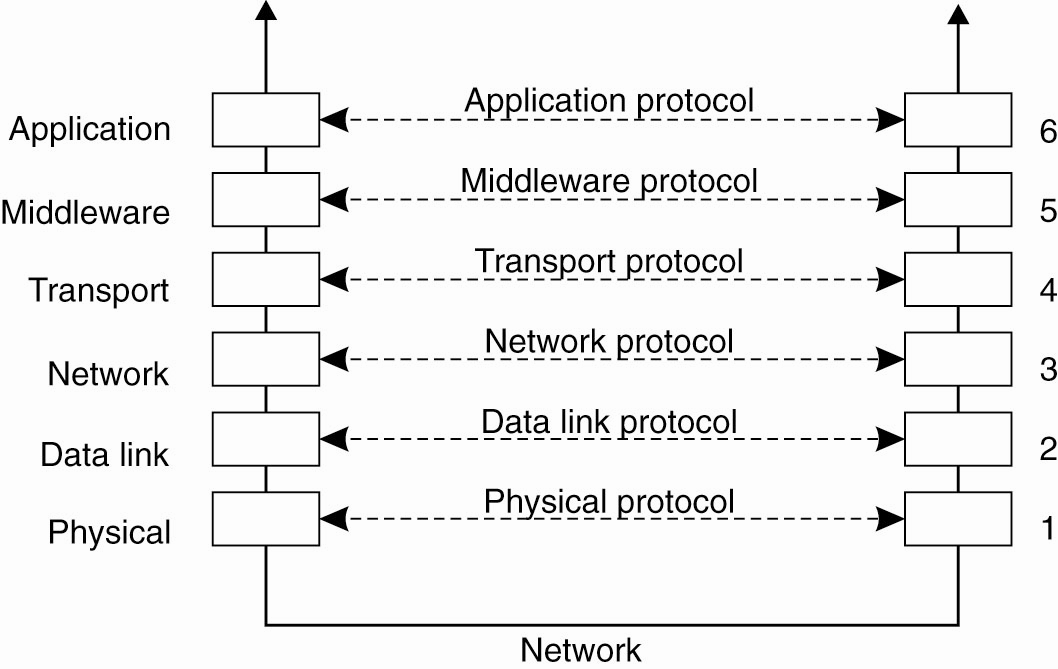
\includegraphics[scale=0.5]{img/osimid.png}
\caption{Modello OSI-Middleware}\label{img:osimid}
\end{figure}
\subsubsection{Tipi di comunicazione}
Esistono diverse alternative nella comunicazione che il middleware mette a disposizione delle applicazioni; partiamo dall'esempio mostrato in \figurename\,\ref{img:midcomuni}. In questo caso possiamo pensare che ogni \emph{host} esegua uno \emph{user agent} ovvero un processo che esegue le operazioni di comunicazione tra i vari sistemi.\\
\begin{figure}
\centering
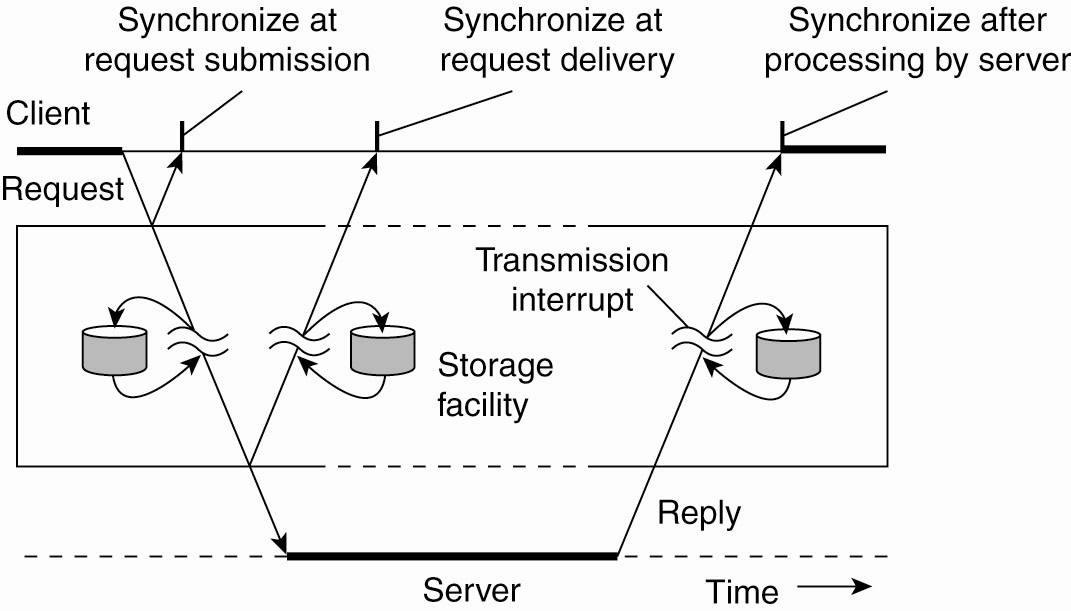
\includegraphics[scale=0.5]{img/midcomuni.png}
\caption{Esempio di tipi di comunicazione}\label{img:midcomuni}
\end{figure}
Prendiamo ora come esempio il caso di un invio di e-mail in questo caso i due \emph{user agent} saranno rispettivamente il sistema che invia e quello che riceve le e-mail. L'agente dal lato del mittente passa la mail al sistema per la consegna delle mail nella convinzione che tale sistema consegni la mail, l'agente dal lato del destinatario a sua volta si connette al sistema per sapere se è giunta qualche nuova mail in caso affermativo la mail viene trasferita dal sistema allo user agent del destinatario.\\
Questo tipo di meccanismo è detto \textbf{comunicazione persistente} in quanto il messaggio viene memorizzato dal middleware per tutto il tempo necessario affinché la consegna non vada a buon fine durante questo periodo non è necessario che i due elementi siano in esecuzione contemporaneamente. Nel caso di \textbf{comunicazione transiente} invece, il sistema memorizza i messaggi scambiati solo finché sia il mittente che il destinatario sono in esecuzione.\\
Oltre che persistente o transiente una comunicazione può essere asincrona o sincrona. Si parla di comunicazione \textbf{asincrona} quando il mittente continua la sua elaborazione subito dopo l'invio del messaggio. Nel caso di comunicazione \textbf{sincrona}, invece, il mittente è bloccato fino a quando la sua richiesta non viene accettata. Ciò può avvenire fino a quando il middleware non comunica la presa in consegna della richiesta, oppure quando la richiesta non viene consegnata al destinatario l'ultima possibilità è che il mittente resta bloccato fino alla fine dell'elaborazione da parte del destinatario e invio di una risposta all'elaborazione.\\
Esistono molti tipi in cui combinazione persistente, transiente, sincrona e asincrona possono essere combinati ma le più diffuse sono la persistenza e la sincronizzazione, la transiente con la sincronizzazione alla fine dell'elaborazione.\\
Dobbiamo distinguere, infine tra comunicazione discreta e a \emph{stream}.
\subsection{Chiamate a procedure remote}
Molti sistemi si basano sullo scambio di messaggi esplicito tra processi, questo scambio avviene tramite l'utilizzo delle procedure \texttt{send} e \texttt{recive} che però non nascondono del tutto la comunicazione. Una nuova tecnica fu introdotta nel 1984 quando si pensò di permettere ai programmi di richiamare procedure situate su altre macchine. Quando un processo sulla macchina $A$ richiama una procedura sulla macchina $B$ il processo chiamante viene sospeso e ha luogo l'elaborazione sulla macchina $B$. Le informazioni sono passate dal chiamante al chiamato tramite i parametri e ritornano indietro come risultato della procedura. Questo tipo di meccanismo è conosciuto come \textbf{chiamata a procedura remota } o \textbf{RPC} (\emph{remote procedure call}).\\
Sebbene l'idea di base risulti molto semplice i problemi relativi sono molti, primo fra tutti visto che chiamante e chiamata risiedono su due macchine diverse lo spazio degli indirizzi è completamente diverso, inoltre, il passaggio di parametri e dei risultati non è così semplice in quanto le macchine potrebbero avere rappresentazione dei dati differenti.
\subsubsection{Operazioni di base sulle RPC}
Iniziamo a vedere come funzionano realmente le RPC partendo dall'analisi di una chiamata a procedura locale per poi analizzare le chiamate remote.
\paragraph{Chiamate a procedura locali}
Per capire come lavorano le RPC è necessario capire comprendere come lavorano le chiamate a procedura convenzionali, ovvero su una singola macchina.
consideriamo una chiamate in C tipo:
\begin{center}
\texttt{count = read(fd, buf, nbytes)}
\end{center}
dove \emph{fd} è un intero che indica un file, \emph{buf} è un array di caratteri e \emph{nbytes} è il numero intero di byte da leggere ed immagazzinare in \emph{buf}.Se la chiamata è stata eseguita dal \emph{main} allora lo \emph{stack} della chiamata sarà quello mostrato in \figurename\,\ref{img:localstack}. Come vediamo nella figura (b) il chiamante inserisce (\emph{push}) i parametri nello stack in ordine inverso. Alla fine dell'esecuzione della procedura il valore di ritorno è posizionato in un registro vengono rimossi i parametri e viene restituito il controllo al chiamante.\\
\begin{figure}
\centering
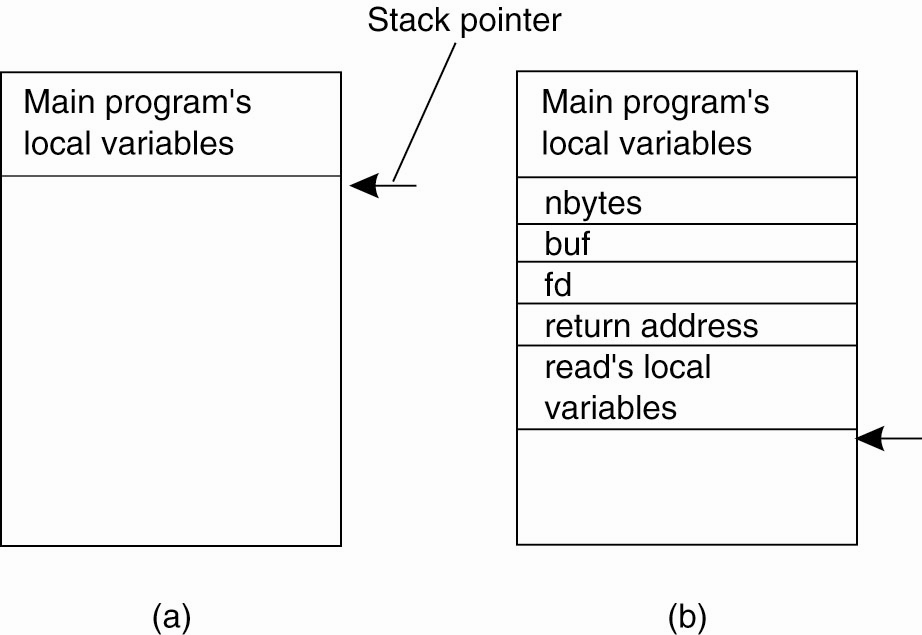
\includegraphics[scale=0.5]{img/localstack.png}
\caption{Stack prima e dopo la chiamata di una procedura}\label{img:localstack}
\end{figure}
Notiamo ora che in C i parametri possono essere passati per \textbf{valore} come \emph{fd} e \emph{nbytes} per i quali il valore viene copiato nello stack o per \textbf{referenza} come nel caso di \emph{buf} il quale è un puntatore ad un array di char; in questo caso nello stack della chiamata non vi è il valore dell'array ma semplicemente un indirizzo che indica dove l'array è situato. Nel caso in cui la procedura modifichi i valori contenuti nell'array tali cambiamenti saranno effettivi anche all'uscita dalla procedura.\\
Esiste un terzo meccanismo di passaggio dei parametri anche se non è usato in C ed è quello per \textbf{copia/ripristino}, questo passaggio consiste nel copiare il valore della variabile nello stack come nel caso di passaggio per valore, e quindi ricopiarla al termine della chiamata sovrascrivendo il valore originale. 
\paragraph{Client e server stub}
L'idea di base delle RPC è quella di rendere le chiamate a procedura remote il più simile possibile ad una chiamata locale. Vogliamo che le RPC siano trasparenti alla distribuzione. Per ottenere tale trasparenza quando il linker assembla il codice al posto di mettere la versione di sistema della procedura, nel nostro caso la \texttt{read}, esso la sostituisce con una versione chiamata \textbf{client stub}. Come quella originale anche questa versione viene richiamata usando la sequenza di \figurename\,\ref{img:localstack}, anche questa esegue una chiamata di sistema, ma a differenza di quella tradizionale questa chiamata impacchetta i dati in un messaggio e ne richiede l'invio al server tramite una \texttt{send}. Dopo l'invio il \emph{client stub} richiama la procedura \texttt{receive} e si blocca in attesa della risposta come mostrato in \figurename\,\ref{img:stub}.
\begin{figure}
\centering
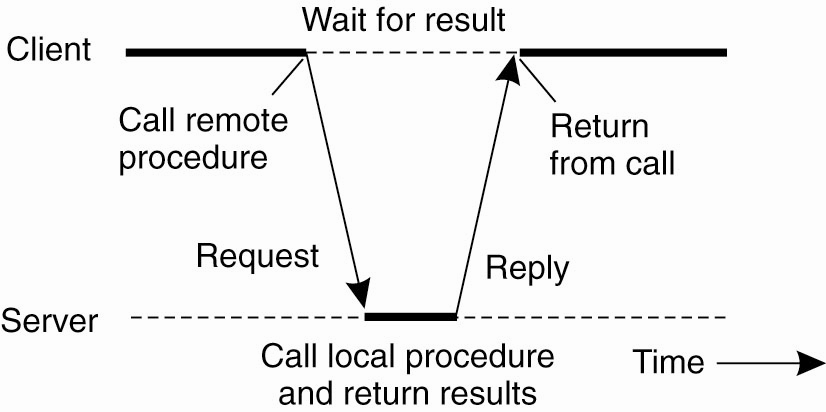
\includegraphics[scale=0.55]{img/stub.png}
\caption{Esempio di chiamata a procedura remota}\label{img:stub}
\end{figure}
Quando il messaggio raggiunge il server esso lo passa al \textbf{server sub}, l'equivalente lato server del \emph{client stub}, questo pezzo di codice trasforma la RPC in una chiamata a procedura locale. Il server esegue il proprio lavoro e restituisce il risultato al chiamante. Quando il \emph{server stub} riprende il controllo impacchetta il risultato in un messaggio e richiama la \texttt{send} per inviare la risposta al client e si rimette in attesa dell'arrivo di una nuova richiesta con la \texttt{receive}. Quando il messaggio di risposta arriva alla macchina client il sistema operativo lo indirizza al \emph{client stub} che lo spacchetta, copia i dati nel buffer e restituisce il controllo al processo client.\\
Quando il client riprende il controllo non ha idea di che cosa sia avvenuto e non ha idea se la chiamata è stata eseguita remotamente o in locale.
Ricapitolando una chiamata a procedura remota segue i seguenti passi:
\begin{enumerate}
\item la procedura client richiama il \emph{client stub} nel modo normale;
\item il \emph{client stub} costruisce un messaggio e richiama il sistema operativo locale;
\item il SO del client invia il messaggio al SO remoto;
\item il SO remoto passa il messaggio al \emph{server stub};
\item il \emph{server stub} spacchetta i parametri e richiama il server;
\item il server esegue il lavoro e restituisce il risultato allo \emph{stub};
\item il \emph{server stub} lo impacchetta in un messaggio e richiama il su SO;
\item il SO del server invia il messaggio al SO del client;
\item il SO del client passa il messaggio al \emph{client stub};
\item lo \emph{stub} spacchetta il risultato e lo restituisce al client.
\begin{figure}
\centering
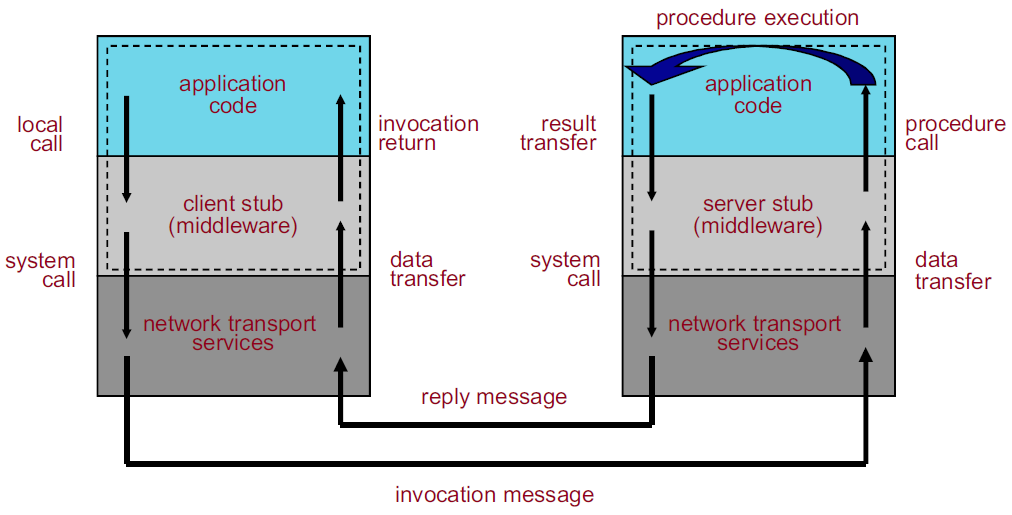
\includegraphics[scale=0.5]{img/execution.png}
\caption{Esecuzione di una chiamata a procedura a procedura remota}\label{img:executionrpc}
\end{figure}
\end{enumerate}
\subsubsection{Passaggio di parametri}
La funzione del client stub è quella di prendere i propri parametri di impacchettarli e di inviarli al server stub. Il problema è che questa operazione pur sembrando molto semplice in realtà non lo è.
\paragraph{Passaggio di parametri per valore}
L'operazione di impacchettare i parametri in un messaggio è detta \textbf{marshaling dei parametri}. Come esempio consideriamo una procedura remota molto semplice come \texttt{add(i,j)} che prende in ingresso due valori interi $i,j$ e restituisce la loro somma aritmetica. L'esecuzione di questa procedura è mostrata in \figurename\,\ref{img:marshal}, nella parte sinistra vediamo la chiamata a tale procedura. Il \emph{client stub} prende i due parametri e li mette in un messaggio semplicemente copiando i valori; insieme ai parametri viene anche inserito il nome (o il numero) della procedura da chiamare in quanto il server potrebbe supportare diverse chiamate. Quando il messaggio raggiunge il server lo \emph{stub} lo esamina per capire quale procedura è richiesta e quindi esegue la chiamata a tale procedura. La chiamata alla procedura è una normale chiamata locale l'unica differenza è che i parametri che vengono passati sono stati estratti dal messaggio e inizializzati nello spazio degli indirizzi dello \emph{stub}.\\
Quando il server ha completato l'esecuzione il controllo ritorna al \emph{server stub} il quale preleva il risultato e lo inserisce nel messaggio di ritorno al \emph{client stub} il quale effettua \emph{unmarshal} e restituisce il risultato al client.\\
\begin{figure}
\centering
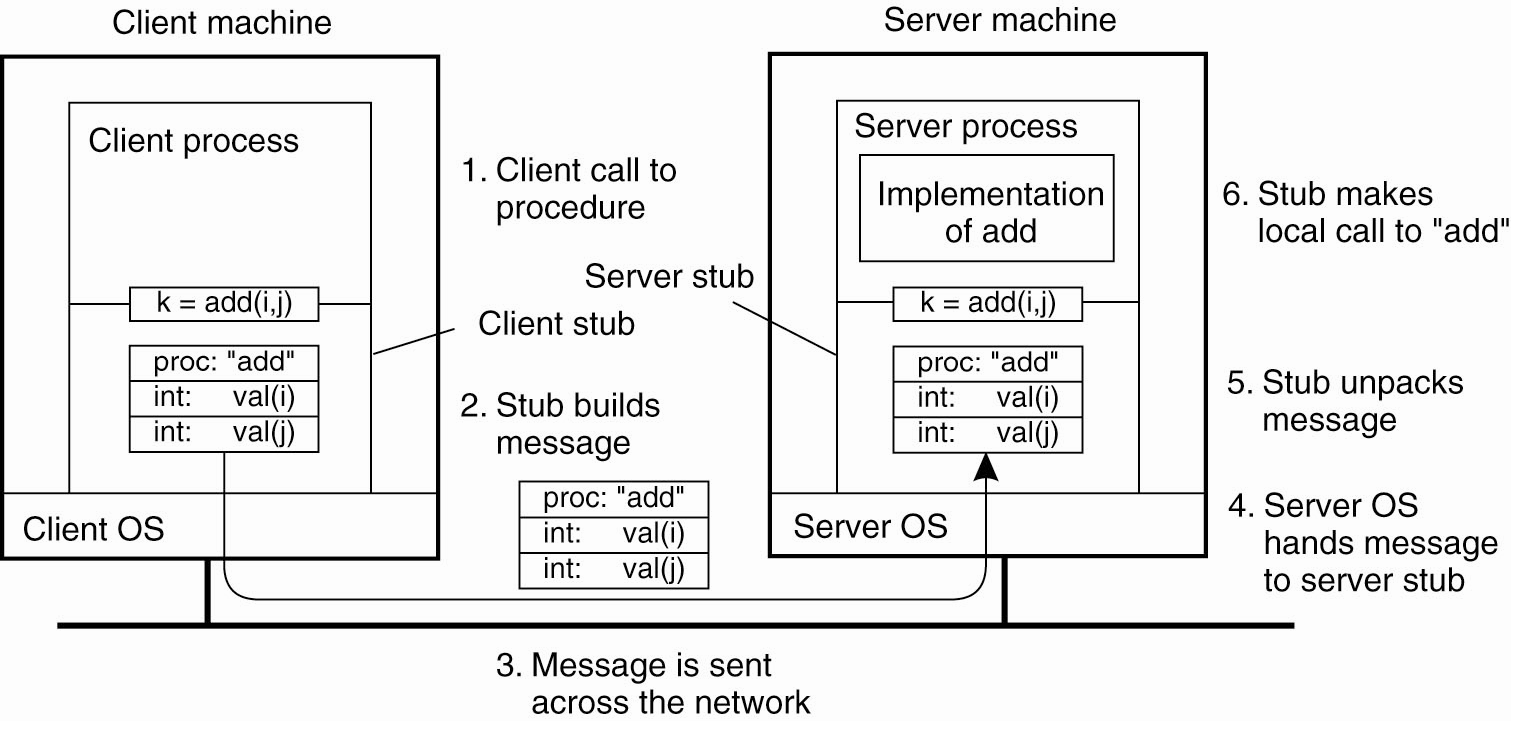
\includegraphics[scale=0.35]{img/rpcparam.png}
\caption{Passaggio di parametri ad una procedura remota}\label{img:marshal}
\end{figure}
I problemi iniziano a sorgere quando due macchine non sono dello stesso tipo, ad esempio i \emph{mainframe IBM} usano una codifica \emph{EBCDIC} per i caratteri mentre i personal computer usano l'\emph{ASCII}; problemi simili possono verificarsi con la rappresentazione degli interi o dei numeri in virgola mobile, in quanto alcune macchine utilizzano la numerazione \textbf{little endian} (numerazione dei bit da destra a a sinistra) altre invece utilizzano la \textbf{big endian} (numerazione da sinistra a destra).
\paragraph{Passaggio di parametri per referenza}
Abbiamo visto il passaggio di parametri per valore, che a parte i problemi di rappresentazione non solleva grosse problematiche. Vediamo ora invece il passaggio di parametri tramite puntatori o riferimenti in generale.\\
Un puntatore ha senso solo nello spazio degli indirizzi del processo in cui è usato. Ad esempio nel  caso della \texttt{read} visto in precedenza il secondo parametro è un puntatore ad un array di caratteri e contiene quindi l'indirizzo al primo elemento dell'array (ad esempio 1000). Se noi passassimo al server tale indirizzo non avrebbe alcun senso in quanto lato server l'indirizzo 1000 potrebbe essere occupato da una istruzione del programma.
La strategia più semplice in questo caso è che il client stub, visto che conosce sia la tipologia che la dimensione dell'array, faccia una copia dell'array nel messaggio e lo invii al server stub il quale a questo punto può richiamare la procedura utilizzando come indirizzo quello dell'aria di memoria nella quale il server stub ha posizionato l'array appena giunto. Quando il server termina il server stub copia nuovamente l'array nel messaggio e lo restituisce al client. Quando il messaggio giunge al client stub esso applica le modifiche all'array originale. Il meccanismo di passaggio per riferimento è stato così sostituito da un meccanismo di \textbf{copia/ripristino}.\\
Esistono delle ottimizzazioni per rendere più efficace tale meccanismo, se gli \emph{stub} conoscono se il parametro è un input oppure un output per il server una delle due copie può essere eliminata.
Abbiamo visto come passare un dato di cui conosciamo la dimensione, nel caso più generale di dati come strutture o oggetti i dati possono essere passati come uno stream di byte, questo meccanismo è chiamato \emph{serializzazione}.
\paragraph{Specifica dei parametri e generazione degli stub}
Come abbiamo visto fino ad ora per nascondere una chiamata remota bisogna che il chiamante e il chiamato concordino sul formato dei messaggi e che eseguano gli stessi passi, in altre parole entrambi i lati di una RPC devono seguire lo stesso \emph{protocollo}. Definire il formato dei messaggi non è però sufficiente è necessario anche che il client e il server concordino sulla rappresentazione delle strutture dati e su come i messaggi debbano essere scambiati, come ad esempio utilizzare un protocollo orientato alla connessione come il TCP/IP.\\
Una volta che il protocollo è stato definito bisogna implementare gli stub, fortunatamente questi differiscono soltanto per le loro interfacce verso le applicazioni .
Per semplificare le cose le interfacce sono spesso definite tramite un \textbf{linguaggio per la definizione di interfacce} (IDL \emph{interface definition language}). Un'interfaccia specificata tramite IDL viene successivamente compilata in un \emph{client stub} e in un \emph{server stub} unitamente alle interfacce \emph{compile-time} o \emph{run-time}.\\
Utilizzare un linguaggio per la definizione delle interfacce semplifica considerevolmente le applicazione client-server basate su RPC.
\subsubsection{RPC in pratica}
Abbiamo visto fino ad ora la teoria che sta dietro ad una chiamata a procedura remota, vediamo ora invece come viene implementato nella realtà un sistema basato sulle RPC.\\
Esistono due vie per produrre un sistema che sfrutta le chiamate a procedura remote, il primo è lo standard \emph{de facto} ed è stato introdotto dalla Sun Microsystem. Questo sistema è parte del Network File System dei sistemi UNIX e specifica il formato dei dati tramite un XDR (\emph{eXternal Data Representation}), il protocollo di trasporto utilizzato è indifferentemente il TCP o UDP, il passaggio di parametri è consentito solo tramite copia e con un massimo di un input ed un output per funzione, infine tale meccanismo fornisce dei meccanismi per la criptazione dei dati.\\
Il secondo meccanismo è quello proposto dall'Open Group ed è chiamato \emph{Distributed Computing Environment} (DCE) ed è un insieme di specifiche e riferimenti. Esistono diverse specifiche per la chiamata di una procedura:
\begin{itemize}
\item \textbf{At-Most-Once:} in cui una chiamata non viene portata avanti più di una volta
\item \textbf{Idempotent:} in questo caso la procedura può essere ripetuta più di una volta senza problemi
\item \textbf{Broadcast:} marcando una procedura in questo modo la richiesta sarà inoltrata a tutte le macchine della rete
\end{itemize}
Come primo passo per creare un'applicazione distribuita dopo aver scelto i meccanismi è quello di chiamare i programmi \emph{uuidgen} i quali generano un prototipo di file IDL contente un identificatore d'interfaccia. A questo punto si completano i file IDL compilando i nomi delle procedure remote ed i loro parametri. Una volta completato il file IDL viene richiamato il compilatore IDL che genera un file \emph{header} da includere nelle applicazione, il \emph{client stub} e il \emph{server stub}. A questo punto il programmatore deve sviluppare le due applicazioni client e server le quali verranno poi compilate e linkate insieme alle librerie e ai rispettivi client e server stub come mostrato in \figurename\,\ref{img:program}
\begin{figure}
\centering
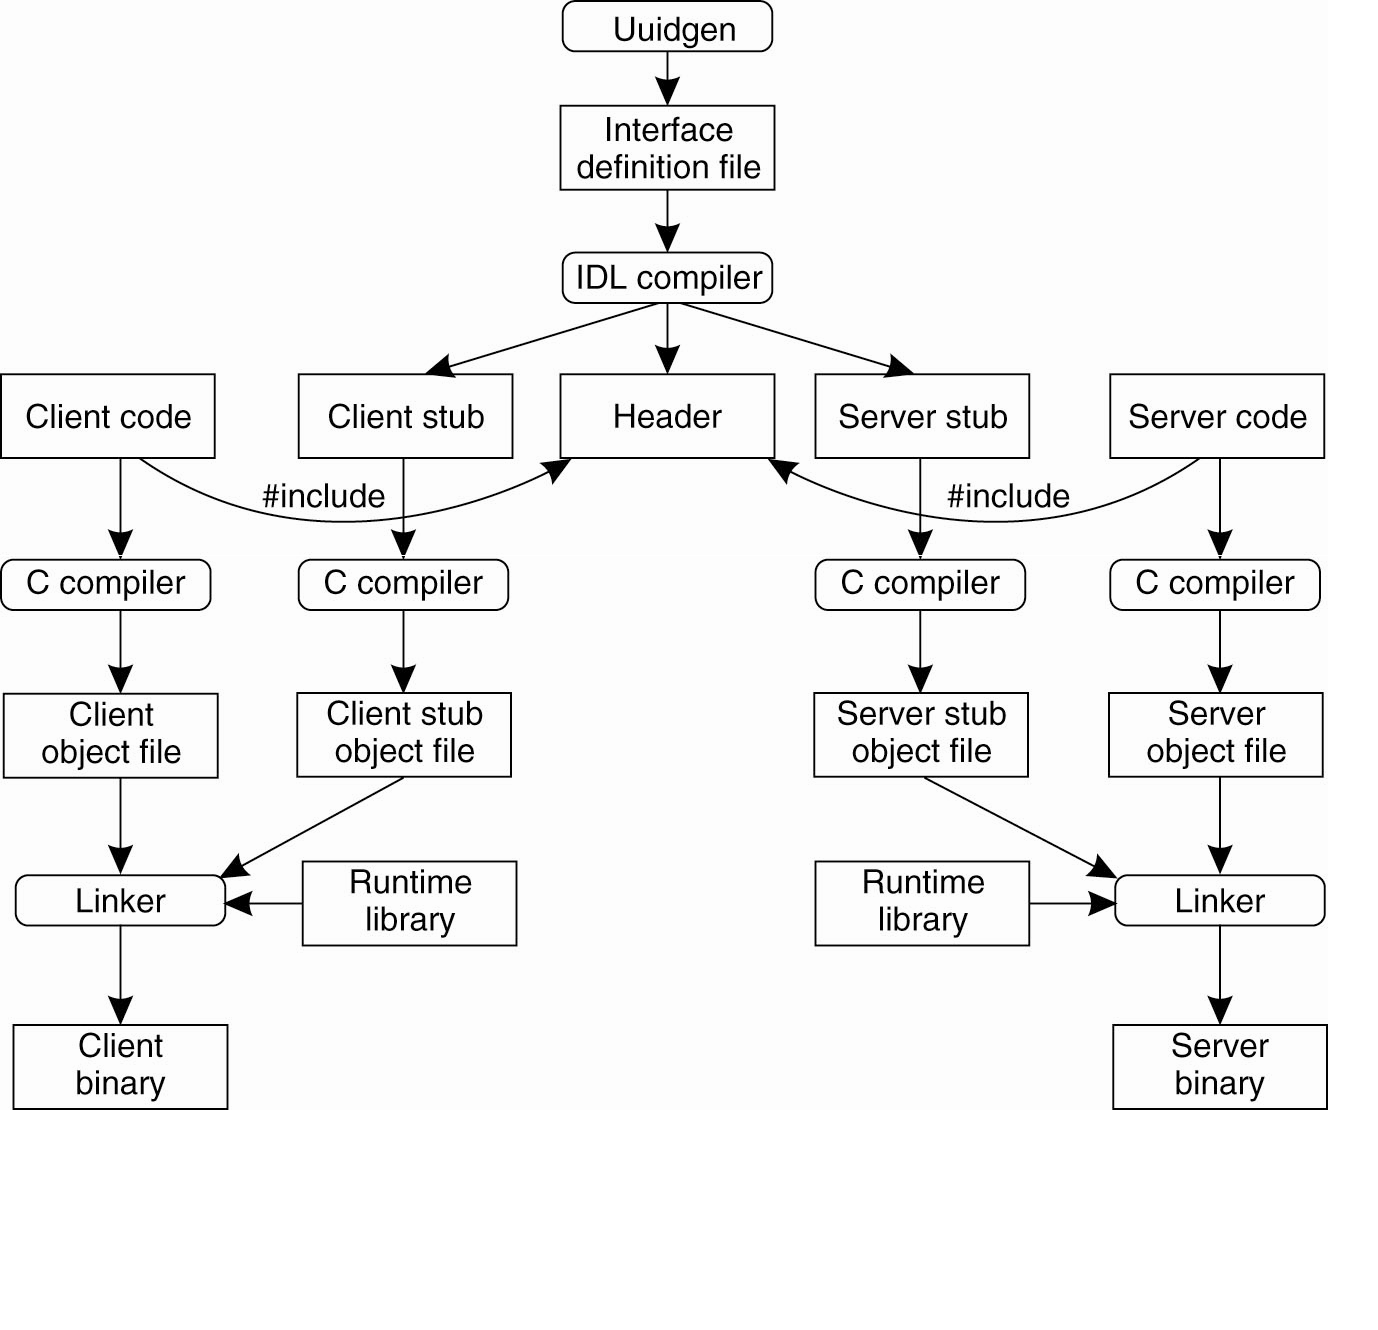
\includegraphics[scale=0.43]{img/program.png}
\caption{Flusso di sviluppo di un'applicazione distribuita}\label{img:program}
\end{figure}
L'ultimo problema che dobbiamo affrontare è come \emph{legare} un client al server che implementa la procedura richiesta dal client. Anche in questo caso Sun e DCE affrontano il problema in due modi differenti. Sun introduce un demone chiamato \texttt{portmap} che associa un server ad una porta, il server occupa una porta disponibile e comunica la sua scelta al \emph{portmap} il client contatta il portmap e richiede la porta necessaria. Il problema principale è che il portmap risolve solo il problema di come stabilire la connessione al server ma deve già conoscere l'ubicazione del server.\\
DCE, invece utilizza due demoni, uno situato sulla stessa macchina del server che svolge la stessa funzione del portmap, ed un secondo demone situato su un server differente (\emph{directory server}) il quale implementa la trasparenza alla distribuzione. Il meccanismo con il quale tale sistema opera è illustrato nella \figurename\,\ref{img:dcebinding}.
\begin{figure}
\centering
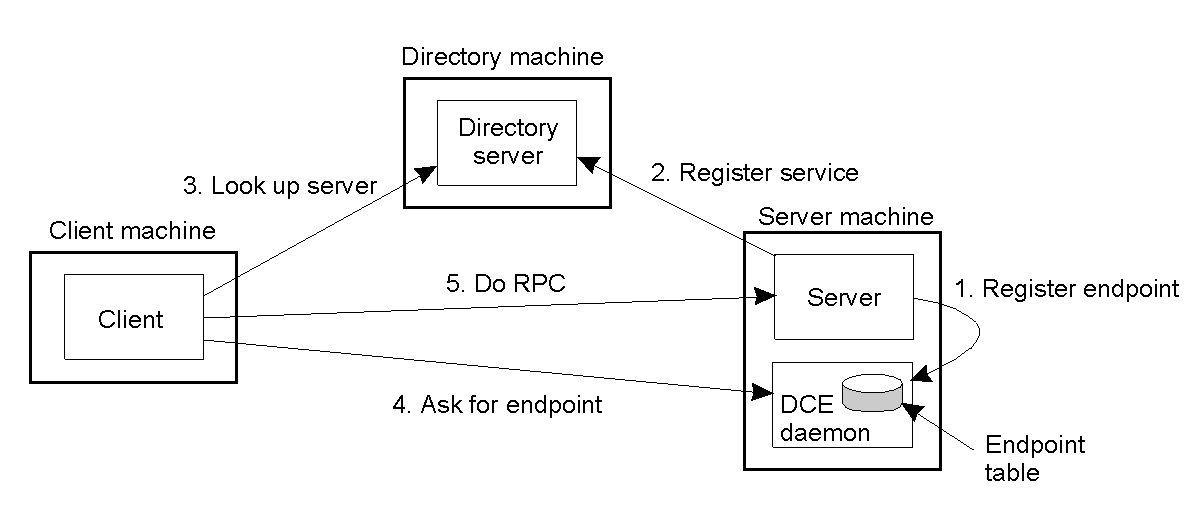
\includegraphics[scale=0.45]{img/dcebinding.png}
\caption{Esecuzioni di un binding tra client e server in DCE}\label{img:dcebinding}
\end{figure}
\subsubsection{Tipi di chiamate a procedure remote}
Fino ad ora abbiamo dato per scontato che le chiamate a procedura remote fossero solamente di tipo sincrono con sincronizzazione alla fine dell'esecuzione della procedura remota. In alcuni casi, però, tale meccanismo non è efficiente in quanto spesso si sprecano risorse lato client. Una possibile variante sono le RPC asincrone le quali possono essere utilizzate quando non sono attesi valori di ritorno e lo sblocco del client avviene all'arrivo di un acknowledgment quando la richiesta viene presa in carico oppure all'arrivo di una \emph{"promessa"} di risposta che verrà inviata tramite un'altra RPC asincrona dal server.\\
La Sun inoltre ha implementato delle RPC \emph{batched} che sono particolari chiamate a procedura che non si aspettano un risultato, queste sono immagazzinate (\emph{buffered}) dal client ed inviate in un unica comunicazione quando si presenta una chiamata non-batched.\\
Un esempio simile avviene nei dispositivi mobili; quando l'host è disconnesso immagazzina le richieste e periodicamente tenta l'invio di richieste, lo stesso viene fatto dal server per l'invio delle risposte. Le richieste e le risposte sono inviate/ricevute su due canali differenti.\\
\subsubsection{Remote method invocation}
Il \emph{Remote Method Invocation} (RMI) è simile alle RPC ma è applicato alla programmazioni ad oggetti, un'importante differenza è che i riferimenti oggetti remoti possono essere passati. L'IDL nel caso di RMI è molto più completo includendo eccezioni ed altro in quanto la separazione tra interfaccia ed implementazione è alla base della programmazione ad oggetti.\\
Le più importanti tecnologie che implementano l'RMI sono \emph{Java RMI} che può essere utilizzata solo implementando in Java ed utilizzando una Java Virtual Machine, è molto semplice e permette il passaggio di parametri sia per riferimento che per valore. \emph{OMG CORBA} è multilinguaggio e multipiattaforma, anche \emph{CORBA} permette il passaggio di parametri sia per riferimento che per valore ma nel secondo caso è compito del programmatore garantire la stessa semantica sia lato server che lato client.
\subsection{Comunicazione orientata agli oggetti}
Le chiamate a procedure remote o le RMI aiutano a nascondere la comunicazione nei sistemi distribuiti, ovvero forniscono un certo grado di trasparenza all'accesso. Tuttavia esistono dei casi in cui questi meccanismi non sono appropriati, come ad esempio nel caso in cui non si è certi che il destinatario  sia attivo nell'istante di invio di un messaggio.La soluzione a queste problematiche sono i \emph{messaggi}.
\subsection{Comunicazione orientata ai messaggi}
Le RPC come abbiamo visto hanno di per se una natura sincrona ed è necessario che sia mittente che destinatario siano in esecuzione all'invocazione della procedura. In molti casi però questo non è possibile o non è conveniente perciò le applicazioni vengono sviluppate utilizzando l'invio di messaggi.
\subsubsection{Comunicazione transiente orientata ai messaggi}
Molti sistemi e applicazioni distribuite sono costruite direttamente in base al semplice modello orientato ai messaggi fornito dal livello di trasporto. Tali applicazioni sono sviluppate attraverso l'utilizzo delle \emph{socket}.
\paragraph{Berkeley socket}
Un'attenzione particolare è stata messa nella standardizzazione dell'interfaccia del livello di trasporto in modo da consentire ai programmatori di far uso dell'intera suit di protocolli attraverso un semplice insieme di primitive.
Una di queste interfacce è \textbf{l'interfaccia socket}introdotta in UNIX Berkeley, un'altra interfaccia importante è la \textbf{XTI (X/open transport interface)}. Le \emph{socket} e XTI sono molto simili nel modello di programmazione ma differiscono nelle primitive.\\
Una socket è una porta di comunicazione su cui un'applicazione può scrivere dati da inviare e da cui poter leggere le risposte.
Le primitive delle socket sono mostrate in \tablename\,\ref{tab:socket}
\begin{table}
\centering
\begin{tabular}{|c|l|}
\hline
\textbf{Primitiva} & \textbf{Significato} \\
\hline
\texttt{Socket} & Crea una nuova porta di comunicazione \\
\texttt{Bind} & Collega un indirizzo locale ad una socket\\
\texttt{Listen} & Annuncia la disponibilità ad accettare connessioni\\
\texttt{Accept} & Blocca il chiamante finché la richiesta di connessione non arriva\\
\texttt{Connect} & Cerca attivamente di stabilire una connessione\\
\texttt{Send} & Invia dati sulla connessione\\
\texttt{Receive} & Riceve dati sulla connessione\\
\texttt{Close} & Rilascia la connessione\\
\hline
\end{tabular}
\caption{Primitive delle socket}\label{tab:socket}
\end{table}
In generale i server eseguono le prime quattro primitive nell'ordine in cui sono presentate. Quando viene richiamata la primitiva \texttt{socket} il chiamante crea una nuova porta di comunicazione ed il sistema operativo locale riserva tale risorsa per la ricezione e l'invio di dati. La primitiva \texttt{bind} associa un indirizzo locale con la socket appena creata, il collegamento (\emph{binding}) indica al sistema operativo che il programma vuole ricevere messaggi solo all'indirizzo e sulla porta specificati. La primitiva \texttt{listen} viene richiamata solo nel caso di comunicazione orientata alla connessione, serve per comunicare al SO quante risorse riservare in base al numero di connessioni massime che il server intende accettare. Tramite la primitiva \texttt{accept} il server si blocca fino all'arrivo di una richiesta di connessione, al suo arrivo il sistema operativo locale crea una nuova \emph{socket} con le stesse proprietà dell'originale e la restituisce al chiamate. Questo meccanismo permette al server di effettuare una \emph{fork} e gestire una comunicazione mentre attende una nuova connessione.\\
Lato client il procedimento è leggermente differente, anche qui è necessario creare la risorsa tramite la primitiva \texttt{socket} ma il \emph{binding} esplicito di tale risorsa non è necessario. La primitiva \texttt{connect} richiede che il chiamante specifichi l'indirizzo a cui va inviata la richiesta di connessione; il client è bloccato fino a quando la connessione non è stata stabilita dopo di che entrambi i lati possono iniziare a scambiarsi messaggi tramite le primitive \texttt{send} e \texttt{receive}. Nelle socket la connessione è simmetrica perciò la chiusura della connessione si ha quando sia il server che il client richiamano la primitiva \texttt{close}.
Il modello generale di una connessione socket è mostrato in \figurename\,\ref{img:socket}.
\begin{figure}
\centering
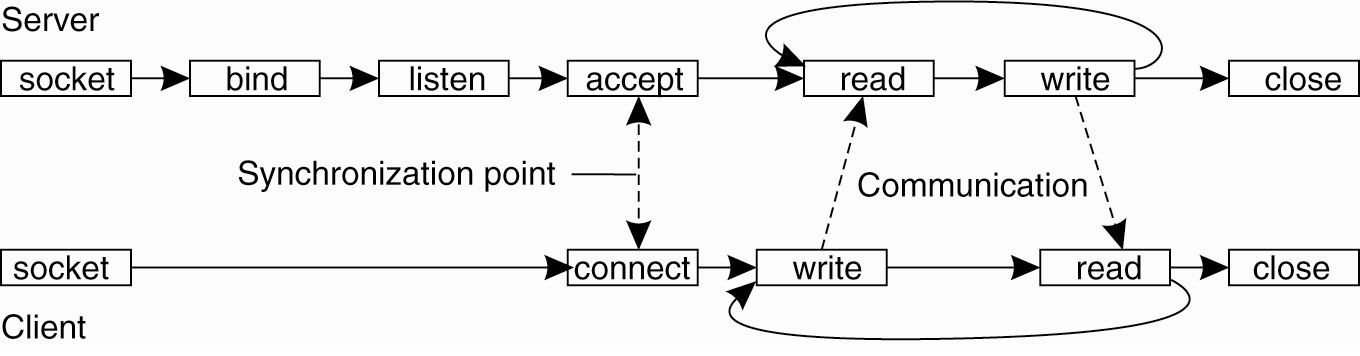
\includegraphics[scale=0.35]{img/sockcon.png}
\caption{Schema generale di una connessione socket}\label{img:socket}
\end{figure}
\paragraph{Interfaccia per lo scambio di messaggi}
Con l'arrivo dei computer ad alte prestazioni gli sviluppatori hanno avuto bisogno di primitive orientate ai messaggi  che consentissero la scrittura di applicazioni in modo facile ed efficiente. Queste caratteristiche fanno si che le primitive siano ad un livello di astrazione sufficientemente alto per sviluppare le applicazioni in modo veloce ma che richiedessero un incremento minimo rispetto alle \emph{socket}, le quali non potevano essere sfruttate in quanto avevano un livello di astrazione troppo basso, ed erano state pensate solo per la comunicazione in rete tramite TCP/IP.\\
Serviva qualcosa che di adatto a reti ad alta velocità come quelle usate nei \emph{cluster} ed inoltre serviva un'interfaccia più avanzata che potesse gestire funzionalità più avanzate come diverse forme di \emph{buffering} e di sincronizzazione.\\
Si è arrivati così alla definizione di uno standard chiamato semplicemente \textbf{interfaccia per lo scambio di messaggi} o \textbf{MPI} (\emph{message-passing interface}). Nato come progetto per le applicazioni parallele e come tale adatto alla comunicazione transiente, utilizza la rete sottostante e presuppone che eventi come la caduta di un processo siano fatali.\\
L'MPI suppone che la comunicazione avvenga tra un gruppo di processi conosciuti, a cui viene assegnato un identificatore  del tipo (\emph{groupID,processID}) che identifica univocamente un processo e che viene utilizzato in sostituzione dell'indirizzo del livello di trasporto.\\
Il cuore di MPI è costituito da primitive per lo scambio di messaggi per supportare la comunicazione transiente, esse sono elencate nella \tablename\,\ref{tab:mpi}
\begin{table}
\centering
\begin{tabular}{|c|l|}
\hline
\textbf{Primitiva} & \textbf{Significato} \\
\hline
\texttt{MPI\_bsend} & Aggiunge un messaggio in uscita a un buffer per l'invio locale \\
\texttt{MPI\_send} & Invia un messaggio e aspetta finché non viene copiato in un buffer\\
\texttt{MPI\_ssend} & Invia un messaggio e aspetta finché non inizia la ricezione\\
\texttt{MPI\_sendrecv} & Invia un messaggio e aspetta la risposta \\
\texttt{MPI\_isend} & Invia il riferimento a un messaggio in uscita e continua \\
\texttt{MPI\_issend} & Invia il riferimento a un messaggio e aspetta finché non inizia la ricezione \\
\texttt{MPI\_recv} & Riceve un messaggio; si blocca se non ce ne sono \\
\texttt{MPI\_irecv} & Controlla se ci sono messaggi in ingresso, ma non si blocca \\
\hline
\end{tabular}
\caption{Elenco delle primitive MPI}\label{tab:mpi}
\end{table}
LA comunicazione transiente asincrona è supportata dalla primitiva \texttt{MPI\_bsend}, il mittente invia un messaggio che viene copiato localmente dal sistema runtime di MPI, quando il messaggio è stato copiato il mittente continua il proprio lavoro. Il sistema runtime locale cancellerà il messaggio dal suo buffer e si occuperà della trasmissione non appena un destinatario chiamerà una \texttt{receive}.\\
Esiste anche un'operazione di invio bloccante, la \texttt{MPI\_send} la quale blocca il chiamante fino a quando il messaggio non è stato copiato nel buffer runtime del destinatario oppure fino a quando il destinatario non ha iniziato la ricezione. La comunicazione sincrona nella quale il mittente si blocca fino a quando la sua richiesta non è accettata avviene tramite la \texttt{MPI\_ssend}, infine, è disponibile anche una comunicazione fortemente sincrona nella quale il sistema attende fino all'esecuzione della richieste e ricezione della relativa risposta che avviene tramite la primitiva \texttt{MPI\_sendrecv}; quest'ultima corrisponde ad una normale RPC.\\
Le due primitive \texttt{MPI\_send} e \texttt{MPI\_ssend} hanno delle varianti che evitano di copiare il messaggio nel buffer locale, queste varianti corrispondono ad un tipo di comunicazione asincrona e si ottengono tramite la \texttt{MPI\_isend} tramite il quale il mittente invia un puntatore ad un messaggio dopodiché il sistema runtime di MPI si occupa della comunicazione mentre il mittente prosegue con la sua esecuzione. La primitiva \texttt{MPI\_issend} fornisce la sicurezza che il destinatario abbia accettato il messaggio e stia lavorando sulla richiesta.\\
Le operazioni \texttt{MPI\_recv} e \texttt{MPI\_irecv} sono rispettivamente le primitive bloccanti e non bloccanti usate per la ricezione dei messaggi.\\
I diversi tipi di comunicazione sono mostrati in \figurename\,\ref{img:tranmpi}.
\begin{figure}
\centering
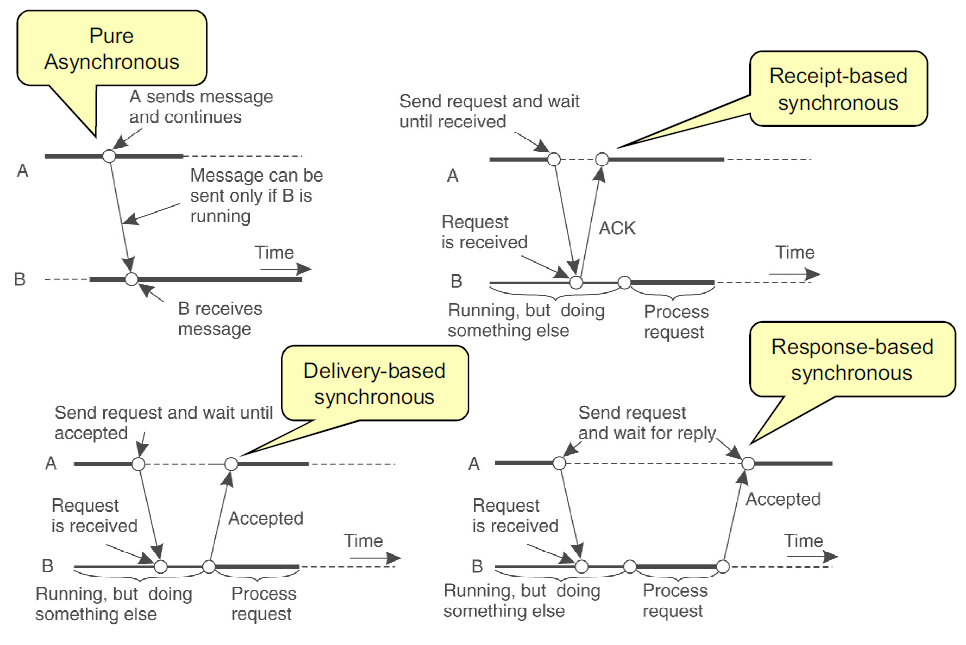
\includegraphics[scale=0.5]{img/tranmpi.png}
\caption{Esempi di comunicazione di tipo transiente}\label{img:tranmpi}
\end{figure}
\subsubsection{Comunicazione persistente orientata ai messaggi}
La classe più importante di servizi middleware orientati ai messaggi è quella conosciuta come \textbf{sistemi a code di messaggi} o semplicemente \textbf{middleware orientati ai messaggi} (MOM, \emph{message oriented middleware}). Questo tipo di sistemi forniscono un ampio supporto alla comunicazione asincrona persistente. La caratteristica fondamentale di questi sistemi è che permettono di memorizzare i messaggi senza che il mittente e il destinatario siano attivi durante la trasmissione del messaggio. 
\paragraph{Modello a code per lo scambio di messaggi}
L'idea di base è che le applicazioni comunicano inserendo i messaggi in code specifiche, questi messaggi vengono poi inoltrati tramite una serie di serve e alla fine consegnati al destinatario.\\
La particolarità è che un mittente non ha la garanzia che un messaggio venga effettivamente letto ma ha solo la garanzia che tale messaggio sarà inserito prima o poi nella coda dei messaggi del destinatario.\\
Questo aspetto fa si che vi sia un forte disaccoppiamento nelle comunicazioni e non vi è quindi la necessità che il destinatario sia in esecuzione quando viene inviato il messaggio, analogamente non vi è la necessità che il mittente sia in esecuzione quando il messaggio viene prelevato dal destinatario come mostrato in \figurename\,\ref{img:asincrono}.
\begin{figure}
\centering
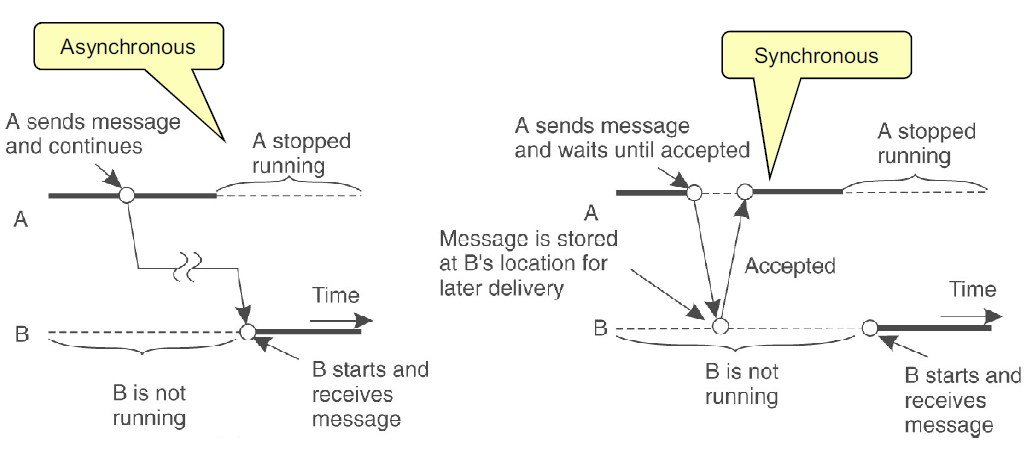
\includegraphics[scale=0.5]{img/asincrono.png}
\caption{Esempio di comunicazione persistente orientata ai messaggi}\label{img:asincrono}
\end{figure}
Questo significa che un messaggio rimarrà in coda fino a quando non verrà rimosso senza tenere conto se il mittente o il destinatario sono in esecuzione.\\
I tipi di messaggi che possono essere inviati sono infiniti, l'unica restrizione è che essi siano opportunamente indirizzati; per l'indirizzamento viene fatto fornendo un nome univoco a livello del sistema della coda di destinazione.
La semplicità di questa architettura si rispecchia anche nella sua interfaccia che è mostrata in \tablename\,\ref{tab:queeue}.
\begin{table}
\centering
\begin{tabular}{|c|l|}
\hline
\textbf{Primitiva} & \textbf{Significato} \\
\hline
\texttt{Put} & Aggiunge un messaggio ad una coda specifica \\
\texttt{Get} & Preleva il primo messaggio in coda nel caso sia vuota si blocca \\
\texttt{Poll} & Preleva il primo messaggio in coda ma non è bloccante \\
\texttt{Notify} & Installa un handler da chiamare quando arriva un messaggio nella coda\\
\hline
\end{tabular}
\caption{Interfaccia di base per una coda in un sistema a code di messaggi}\label{tab:queeue}
\end{table}
La primitiva \texttt{put} viene richiamata da un mittente per passare un messaggio al sistema sottostante e posizionarlo in una coda specifica. La \texttt{get} è una chiamata bloccante attraverso la quale un processo autorizzato può rimuovere dalla coda specificata il messaggio pendente da più tempo; nel caso la coda sia vuota il processo viene bloccato. La corrispettiva chiamata non bloccante è la \texttt{pull}.
Molti sistemi inoltre permettono l'installazione di un \emph{handler} sotto forma di \emph{funzione callback} che viene richiamata all'arrivo di ogni nuovo messaggio; molto utili nel caso si volesse avviare un processo per la ricezione dei messaggi.
\paragraph{Architettura generale di un sistema a code}
In realtà la vera architettura di un sistema a code di messaggi ha alcune restrizioni; prima fra tutti è che i messaggi possono essere inseriti solo in code \emph{locali} al mittente ovvero code sulla stessa macchina o comunque sulla stessa LAN raggiungibile in modo \emph{efficiente} tramite una RPC. Una coda di questo tipo è chiamata \textbf{coda sorgente}.
Analogamente i messaggi possono essere letti soltanto da code locali dette \textbf{code di destinazione}. \uppercase{è} responsabilità del sistema fare in modo che coda sorgente e coda destinazione siano disponibili e che i messaggi vengano recapitati nel modo corretto. \\
L'insieme delle code è distribuito su molte macchine perciò il sistema deve mantenere una corrispondenza tra le code e la loro posizione, questo significa mantenere una base di dati di \textbf{nomi delle code} e delle rispettive posizioni sulla rete come mostrato in \figurename\,\ref{img:queeuename}
\begin{figure}
\centering
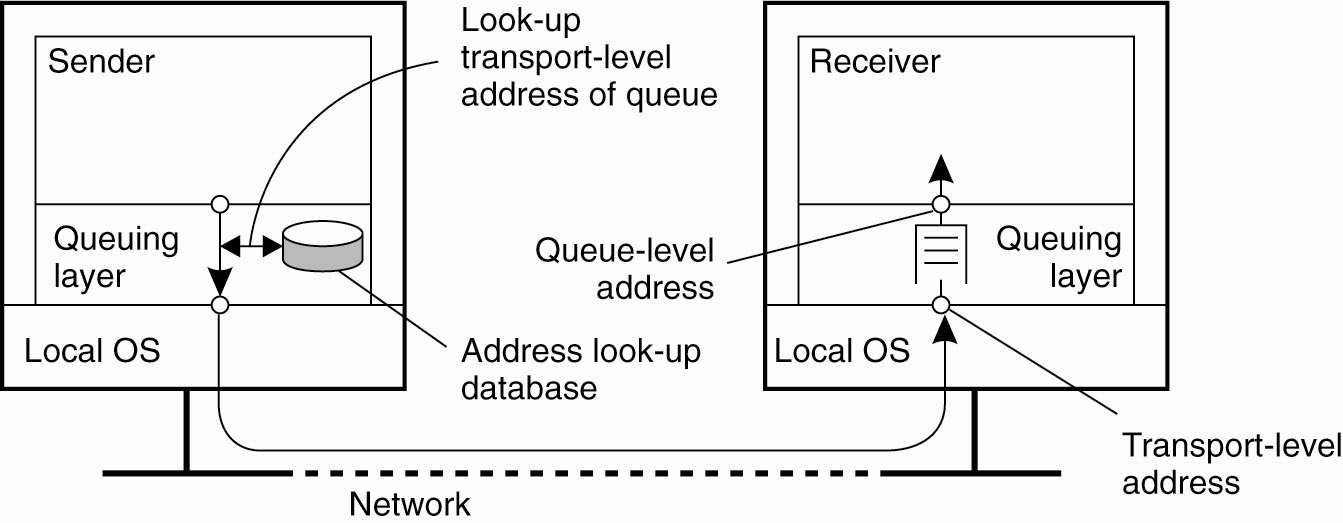
\includegraphics[scale=0.4]{img/queeuename.png}
\caption{Esempio di uso di basi di dati per i nomi delle code}\label{img:queeuename}
\end{figure}
Questo meccanismo è molto simile all'uso del \emph{domain name system} (DNS). Le code sono gestite dai \textbf{gestori delle code} i quali interagiscono direttamente con le applicazioni che inviano e ricevono messaggi; esistono però gestori speciali che agiscono da \emph{router} o \textbf{relay} che inoltrano messaggi in ingresso ad altri gestori. in questo modo un sistema a code può crescere e diventare una rete \textbf{\emph{overlay}} completa basata un una rete di computer esistente.\\
I \emph{relay} possono essere utili per molti motivi, nei sistemi nei quali non è possibile mantenere un \emph{naming server} generale il quale possa mantenere dinamicamente la corrispondenza coda-posizione e la topologia della rete è statica ed ogni gestore delle code deve mantenere una copia della corrispondenze coda-posizione allora in questo caso possono verificarsi problemi di gestione della rete. Una soluzione possibile è quella di utilizzare dei \emph{router} i quali conoscono la topologia della rete. Quando un mittente $A$ inserisce un messaggio per un destinatario $B$ allora il messaggio è trasferito al più vicino \emph{router} chiamato $R1$ come si vede nella \figurename\,\ref{img:queeuerouter}.
\begin{figure}
\centering
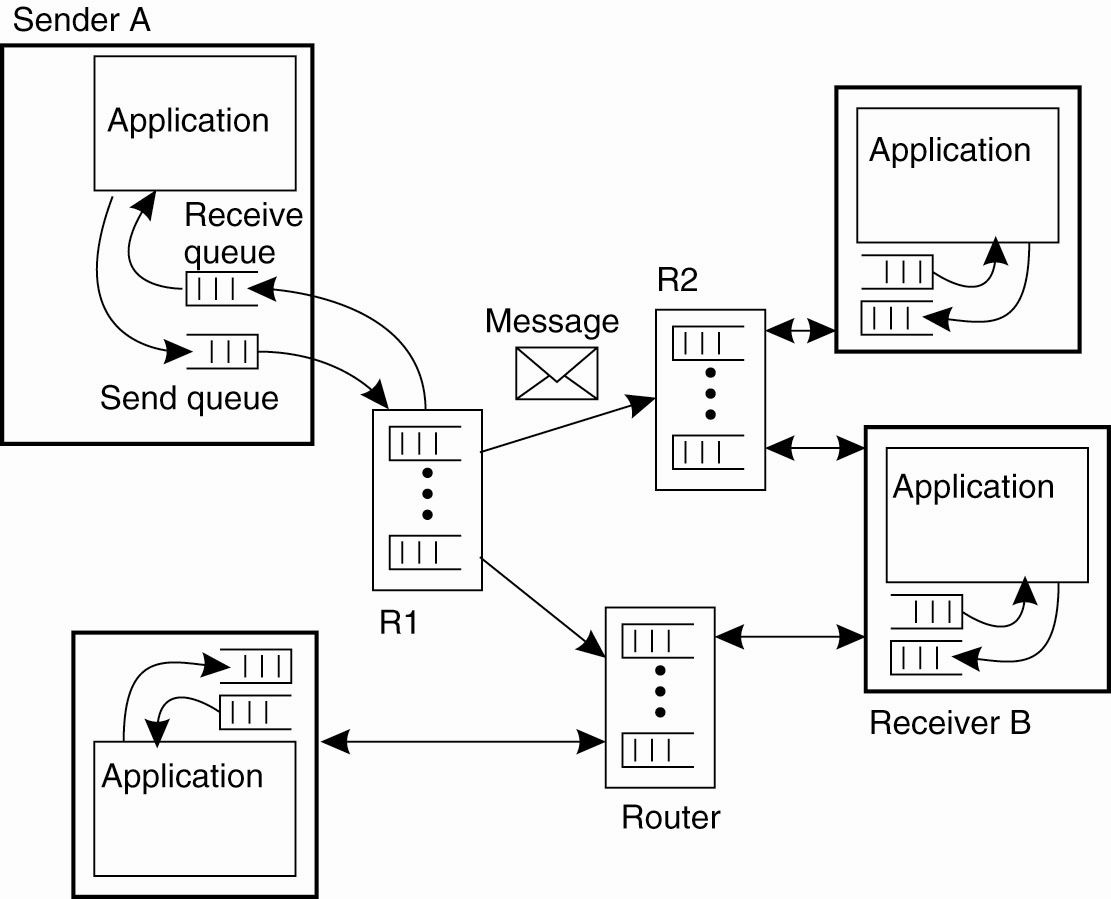
\includegraphics[scale=0.4]{img/queeuerouter.png}
\caption{Organizzazione generale dei sistemi a code di messaggi con \emph{router}}\label{img:queeuerouter}
\end{figure}
A questo punto il router $R1$ potrebbe dedurre da alcune informazioni contenute nel messaggio che la direzione verso la quale inoltrare il messaggio è quella di $R2$. In questo modo è necessario solo aggiornare i router su quali code vengono aggiunte o eliminate mentre i gestori devono solo preoccuparsi di individuare il router più vicino.\\
I \emph{relay} agevolano la costruzione di sistemi a code di messaggi scalabili, tuttavia al crescere della rete diventa impossibile la gestione manuale della rete, la soluzione è quella di adottare sistemi di \emph{routing} dinamici come avviene nelle reti di computer.\\
Un altro vantaggio dei \emph{relay} è quello di consentire un'elaborazione secondaria dei messaggi per ragioni di sicurezza e tolleranza ai guasti; oppure per trasformare i messaggi in una forma comprensibile al destinatario, in questo caso parliamo di \emph{gateway}; infine, i relay possono essere usati per effettuare il \emph{multicasting}.
\paragraph{Broker di messaggi}
Una caratteristica importante dei sistemi a code di messaggi è  la possibilità di integrare applicazioni nuove con alcune già esistenti in un unico sistema distribuito. L'integrazione richiede che tutte le applicazioni del sistema possano interpretare i messaggi che ricevono, questo implica che i messaggi in uscita da un'applicazione siano nello stesso formato di quelli del destinatario.\\
Questa caratteristica non è sempre garantita da tutte le applicazioni. Una soluzione è quella di concordare un \emph{protocollo} comune per tutte le applicazioni ma sfortunatamente tale meccanismo non funziona con i sistemi a code di messaggi in quanto il livello di astrazione è troppo alto e un meccanismo di questo genere ha senso solo se le informazioni da scambiare sono molte.\\
L'altro approccio è quello di provare a convivere con tutti questi formati e fornire un meccanismo di conversione il più semplice possibile. Nei sistemi a code di messaggi tale conversione è gestita da alcuni nodi speciali chiamati \textbf{broker di messaggi}. Un \emph{broker} agisce da \emph{gateway} a livello applicativo, il suo obiettivo è quello di convertire i messaggi in ingresso in modo che siano comprensibili dall'applicazione destinataria.\\
In un sistema a code di messaggi un \emph{broker} non è altro che un'applicazione come si può vedere anche da \figurename\,\ref{img:broker}.\\
\begin{figure}
\centering
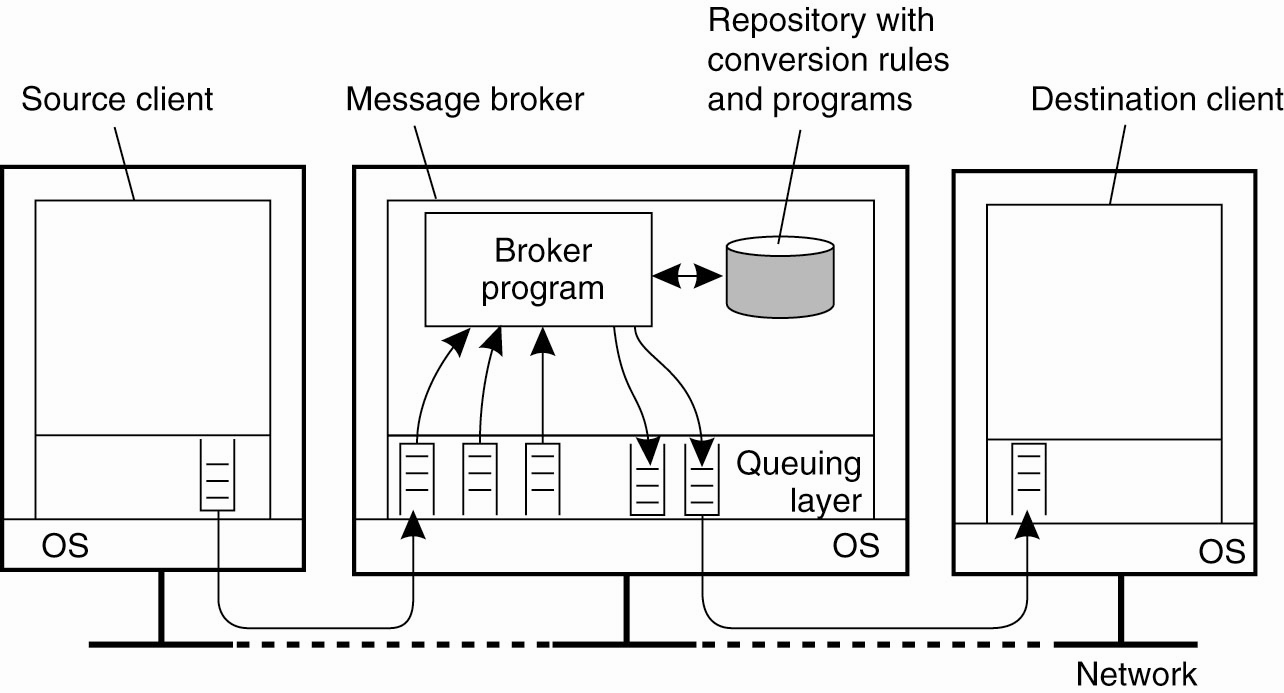
\includegraphics[scale=0.4]{img/broker.png}
\caption{Esempio generale di un broker}\label{img:broker}
\end{figure}
La funzione più comune di un \emph{broker} è quella di effettuare l'\textbf{integrazione di applicazioni aziendali} (EAI,\emph{enterprise application integration}), in questo caso oltre a convertire i messaggi il broker deve trovare una corrispondenza tra le applicazioni basandosi sui messaggi che si sono scambiati. In tale modello, chiamato \textbf{publish/subscribe}, le applicazioni inviano messaggi sotto forma di \emph{publishing} riguardo ad un determinato argomento $X$ al broker, le applicazioni che hanno dichiarato il loro interesse all'argomento $X$ tramite una \emph{subscription} riceveranno questi messaggi dal broker. Esistono due tipologie di sottoscrizioni, la \emph{subject-based} nella quale l'argomento è determinato a priori, oppure, la \emph{content-based} nella quale la sottoscrizione contiene un'espressione (filtro) che permette il filtraggio degli eventi in base al loro contenuto.\\
Il cuore di un broker è il \emph{repository} delle regole e dei programmi che consentono di trasformare un messaggio del tipo $T1$ in un messaggio del tipo $T2$.
\subsubsection{Event dispatcher}
L'\emph{event dispacher} è quel componente che, in un sistema basato sugli eventi, raccoglie le sottoscrizioni e distribuisce gli eventi ai vari client. Questo componente può essere centralizzato, oppure, per ragioni di scalabilità, distribuito; nel caso distribuito un insieme di broker sono organizzati in una rete \emph{overlay} cooperante per raccogliere le sottoscrizioni, la tipologia della rete può essere ciclica o aciclica.\\
Nel caso di rete aciclica ogni broker immagazzina le sottoscrizioni dei client a lui collegati, i messaggi sono scambiati tra i diversi broker e inoltrati ai client solo se si sono sottoscritti.
Per quanto riguarda le sottoscrizioni ogni broker inoltra le sottoscrizioni agli altri ma non viene mai mandata la stessa sottoscrizione due volte sullo stesso collegamento. I messaggi seguono le stesse vie delle sottoscrizioni. In particolare ogni volta che un broker riceve un messaggio esso effettua un matching con un lista di filtri per determinare una lista di inoltro. L'efficienza di questo meccanismo dipende dalla complessità del linguaggio di sottoscrizione e dall'algoritmo di forwarding utilizzato. Il più comune nel caso aciclico è il forwarding di tipo gerarchico; messaggi e sottoscrizioni sono inoltrati verso la radice dell'albero, i messaggi ridiscendono solo se esiste un matching nelle sottoscrizioni lungo il percorso intrapreso.\\
Nel caso di grafo ciclico un sistema di tipo DHT (\emph{distributed hash table}) organizza i nodi in una struttura nella quale il routing è efficiente e avviene nei nodi nei quali si ha un ID più piccolo o al più uguale ad un altro ID.
Le sottoscrizioni a dei messaggi aventi un certo soggetto $S$ vengono così processate:
\begin{itemize}
\item Si calcola l'hash (\emph{Hs}) dell'argomento $S$ 
\item Si utilizza la DHT per inoltrare la sottoscrizione a \emph{succ(Hs)}
\item Durante l'inoltro della sottoscrizione verso $succ(Hs)$ si comunicano delle informazioni ai nodi attraversati per il successivo inoltro dei messaggi.
\end{itemize}
La pubblicazione dei messaggi aventi un certo argomento $S$ vengono così inoltrati:
\begin{itemize}
\item Si calcola l'hash dell'argomento $Hs$
\item Si utilizza la DHT per inoltrare il messaggio al nodo $succ(Hs)$
\item Durante l'inoltro verso $succ(Hs)$ utilizza le informazioni lasciate dalla sottoscrizione per inoltrare il messaggio ai nodi interessati.
\end{itemize}
Per quanto riguarda sistemi \emph{content based} esistono diversi meccanismi sia per il \emph{forwarding} sia per \emph{routing}, per quanto riguarda il forwarding le tecniche utilizzate sono:
\begin{itemize}
\item Per Source Forwarding (PSF)
\item Improved per source forwarding (iPSF)
\item Per receiver forwarding (PRF)
\end{itemize}
Mentre per quanto riguarda il routing solitamente si utilizzano:
\begin{itemize}
\item Distance Vector (DV)
\item Link-State (LS)
\end{itemize}
\paragraph{PSF: Per-Source Forwarding}
Nel caso del PSF si parte da un nodo e si calcola l'albero a cammino minimo; ottenuto quest'albero si riempe una tabella associata ad ogni nodo in questo modo con un campo \emph{sorgente} un campo \emph{successivo} ed un campo \emph{predicato} come mostrato in \figurename\,\ref{img:psf}.
Come \emph{sorgente} si utilizza il nodo radice utilizzato per calcolare lo SPT, come \emph{successivo} si utilizza uno dei nodi figli a quello in cui si sta riempiendo la tabella e nel campo \emph{predicato} si esegue l'operazione di \emph{or logico} sui predicati dei nodi figli.
Nell'esempio di \figurename\,\ref{img:psf} abbiamo che il nodo numero 1 è utilizzato per calcolare l'albero a costo minimo, la tabella che si sta calcolando è quella del nodo 2 i valori successivi sono $\{4,5,8\}$ i predicati che si ottengono sono \emph{Pf} per quanto riguarda 4, \emph{Pg+Pd} per quanto riguarda il nodo 5.
Ricapitolando definendo il grafo $G = (V,E)$ dove $v \in V$ e definendo i predicati di un nodo come $pred(u)$ allora possiamo definire una serie di passaggi per il calcolo del PSF:
\begin{enumerate}
\item Per ogni nodo $v$ si calcola il corrispettivo albero di costo minimo.
\item Per ogni albero partendo dalla radice $v$ si calcolano tutti i figli che chiamiamo $u$.
\item Per ogni $u$ si compila una tabella con tre campi \emph{sorgente}, \emph{next-hop} e \emph{predicato}.
\item In \emph{sorgente} si mette il valore corrente di $v$
\item In \emph{next-hop} si mette uno dei vicini di $u$
\item In \emph{predicato} si effettua la somma logica dei predicati raggiungibili da \emph{next-hop}
\end{enumerate}
\begin{figure}
\centering
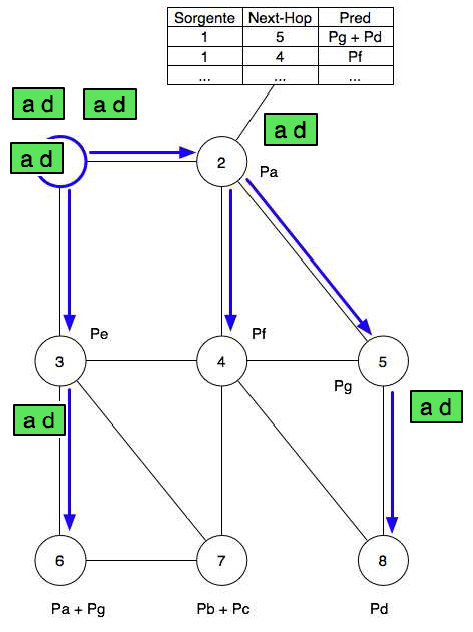
\includegraphics[scale=0.5]{img/psf.png}
\caption{Esempio di PSF}\label{img:psf}
\end{figure}
\paragraph{iPSF: improved PSF}
Il pre-source forwarding implica un grosso dispendio di risorse in quanto le tabelle nei nodi hanno dimensioni molto grandi. Per ottimizzare tale meccanismo si è sviluppato \emph{iPSF} il quale, nel caso in cui due SPT calcolati su due radici diverse hanno un sotto-albero comune allora le tabelle dei nodi del sotto-albero comune avranno come valore del campo \emph{sorgente}, come possiamo vedere in \figurename\,\ref{img:ipsf} dove i nodi 1 e 3 hanno lo stesso sotto albero comune in formato dai nodi $\{2,4,5,8\}$
\begin{figure}
\centering
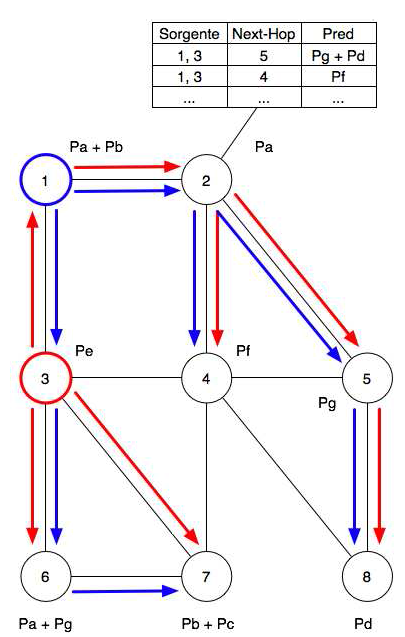
\includegraphics[scale=0.5]{img/ipsf.png}
\caption{Esempio di iPSF}\label{img:ipsf}
\end{figure}
\paragraph{PRF: Per-Reciver Forwarding}
In questo caso il calcolo di chi è interessato al messaggio viene fatto direttamente all'origine e nell'header del messaggio vengono inseriti i nodi interessati. Per ogni nodo esistono due tabelle una che contiene i forwarding con i rispettivi predicati ed un'altra che contiene gli instradamenti ai nodi successi come mostrato in \figurename\,\ref{img:prf}
\begin{figure}
\centering
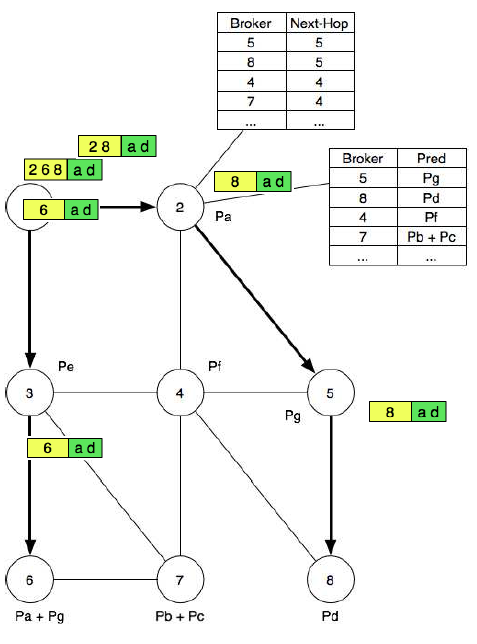
\includegraphics[scale=0.5]{img/prf.png}
\caption{Esempio di PRF}\label{img:prf}
\end{figure}
\paragraph{Algoritmi di routing}
Per quanto riguarda gli algoritmi di routing possiamo averne di due tipi, il primo sono gli algoritmi di tipo \emph{Distance Vector} nei quali i nodi hanno soltanto una visione parziale della rete tramite la richiesta ai nodi vicini del loro stato e la risposta da parte di quest'ultimi, si ha così un algoritmo distribuito nel quale solo col passare del tempo un nodo ha la piena visione della rete. Nel caso degli algoritmi \emph{Link-State} tutti i nodi utilizzano un pacchetto denominato \emph{link-state packet} che viene inoltrato ad un nodo centrale il quale, dopo aver calcolato la rete, restituisce a tutti i nodi le informazioni su tale rete.
\subsection{Comunicazione orientata agli stream}
Fino ad ora abbiamo visto dei meccanismi per lo scambio di informazioni nei quali non ha importanza l'istante in cui avviene tale scambio. Esistono però forme di comunicazione in cui il tempo ha un ruolo fondamentale, come nel caso degli \emph{stream} audio nei quali per riprodurre un suono è necessario che i dati, nel caso stiamo parlando di un CD, siano riprodotti nell'ordine corretto e con una cadenza di 1/44100 sec. Eseguirli ad una velocità diversa riprodurrebbe un suono completamente diverso.
\subsubsection{Supporto ai media continui}
Il supporto allo scambio di informazioni dipendenti dal tempo spesso si traduce nel supporto ai media continui ovvero quei mezzi nei quali viene convogliata l'informazione come media media per la memorizzazione e la trasmissione o media per la presentazione. La caratteristica più importante dei media è come essi \emph{rappresentano} l'informazione. Gli \emph{stream} audio ad esempio possono essere codificati tramite campioni a 16 bit usando la PCM (\emph{pulse code modulation}). Nei \textbf{media continui} le relazioni temporali tra i diversi dati sono fondamentali per interpretare correttamente l'informazione in essa contenuta. Ad esempio il movimento può essere rappresentato da una serie di immagini successive visualizzate ad un intervallo di tempo $T$ regolare pari a 30-40 msec.
\paragraph{Stream di dati}
Per gestire lo scambio di informazioni continue i sistemi distribuiti forniscono supporto agli \textbf{stream di dati}. Uno stream non è altro che una sequenza continua di dati. Gli stream possono essere usati sia per i media continui che per quelli discreti, un esempio di stream di dati discreto sono le connessioni TCP/IP (stream di byte).\\
Il tempo è fondamentale negli stream di dati continui, nella modalità di trasmissione \textbf{asincrona} i dati di uno stream vengono trasmessi in sequenza uno dopo l'altro ma è l'unico vincolo imposto, questo è solo il caso degli stream di dati discreti. \\
Nella modalità di trasmissione \textbf{sincrona} viene definito un tempo massimo di trasmissione per ogni unità di dati in uno stream. Non è importante se un'unità è trasferita più velocemente del tempo massimo.
Esiste infine una modalità di trasmissione \textbf{isocrona} nella quale è necessario che i dati siano trasferiti in un certo tempo. Ciò significa che i dati sono soggetti a vincoli di tempo sia minimi che massimi, questi limiti sono chiamati \emph{bounded (delay) jitter}, questa modalità è abbastanza importante per i sistemi multimediali in quanto ha un ruolo importante nella rappresentazione audio e video.\\
Possiamo fare un'altra distinzione negli stream, essi possono essere \textbf{semplici} quando la sequenza di dati è unica, oppure \textbf{complessi} quando più stream semplici sono in relazione, tali stream sono chiamati \textbf{substream}. La relazione tra \emph{substream} di uno stream complesso dipende spesso dal tempo. L'importante è che i \emph{substream} siano continuamente sincronizzati. In altre parole le unità di dati provenienti da due substream devono essere trasmessi in coppia. Un possibile esempio di architettura di un sistema distribuito multimediale è quello mostrato in \figurename\,\ref{img:stream}.
\begin{figure}
\centering
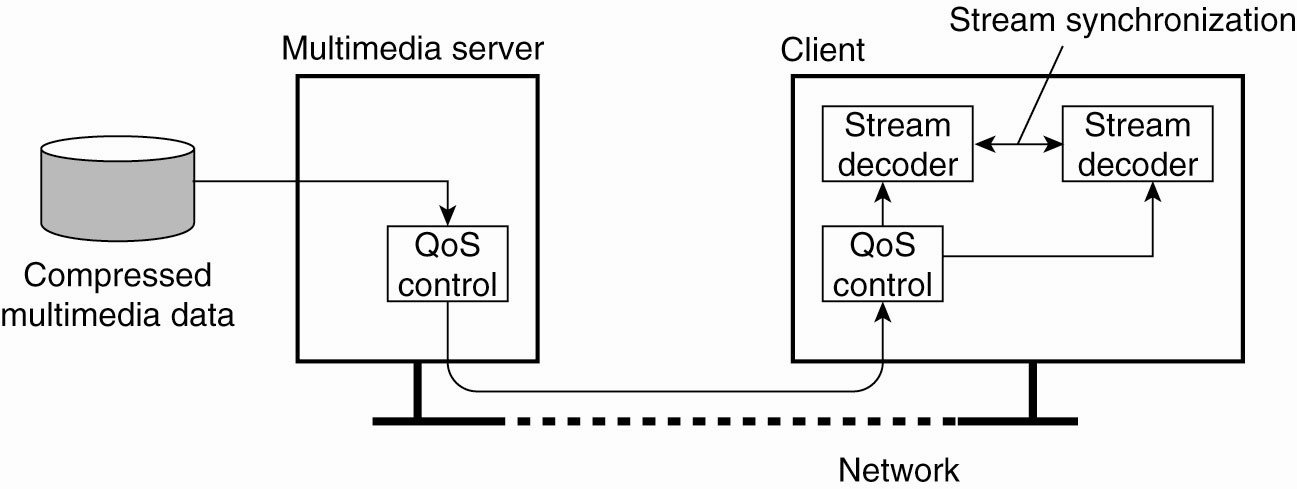
\includegraphics[scale=0.4]{img/stream.png}
\caption{Esempio di sistema multimediale}\label{img:stream}
\end{figure}
\subsubsection{Stream e qualità del servizio}
I requisiti di tempo sono spesso espressi come requisiti della \textbf{qualità del servizio} (\textbf{QoS},\emph{quality of service}). Questi requisiti descrivono che cosa necessiti il sistema per assicurare che i vincoli siano rispettati. La QoS per gli stream di dati continui è essenzialmente relativa al tempo, al volume e all'affidabilità questo significa specificare:
\begin{itemize}
\item il \emph{bit rate} a cui devono essere trasportati i dati;
\item il tempo massimo di \emph{set up} di una sessione (quando un applicazione può iniziare ad inviare dati);
\item il tempo di trasporto massimo;
\item la varianza massima del tempo di trasmissione o \emph{jitter};
\item il tempo massimo di risposta.
\end{itemize}
Tuttavia la maggior parte dei sistemi distribuiti orientati agli stream è costruita sullo stack IP il quale è costituito da un servizio \emph{datagram} di tipo \emph{best-effort}  il quale permette di cancellare pacchetti ogni qual volta la comunicazione diviene troppo pesante.
\paragraph{Garantire la QoS}
Visto i problemi introdotti dall'utilizzo del protocollo IP il sistema distribuito può cercare di sopperire alla mancanza di qualità del servizio.\\
Prima di tutto l'IP permette di differenziare delle classi di dati per mezzo dei suoi \textbf{servizi differenziati}. Ad esempio un host può marcare i suoi pacchetti come appartenenti alla classe di \textbf{inoltro rapido} che indica che il pacchetto deve essere inoltrato dal router con priorità assoluta. Inoltre esiste una classe di \textbf{inoltro assicurato}.\\
Oltre a soluzioni a livello di rete, anche un sistema distribuito può usare alcuni accorgimenti per migliorare le prestazioni. Uno di questi è l'utilizzo di \emph{buffer} per ridurre lo \emph{jitter}; il principio è semplice ed è mostrato in \figurename\,\ref{img:buffer}; il meccanismo prevede la memorizzazione dei pacchetti per un certo tempo massimo prima di passare i pacchetti all'applicazione in modo da avere sempre dei pacchetti a disposizione. Ovviamente può succedere che alcuni pacchetti arrivino con un ritardo maggiore del tempo di buffer questo causerà dei vuoti nello stream. Una soluzione è quella di aumentare il tempo di buffer ma questo causa un aumento del tempo di \emph{set-up} dell'applicazione.\\
\begin{figure}
\centering
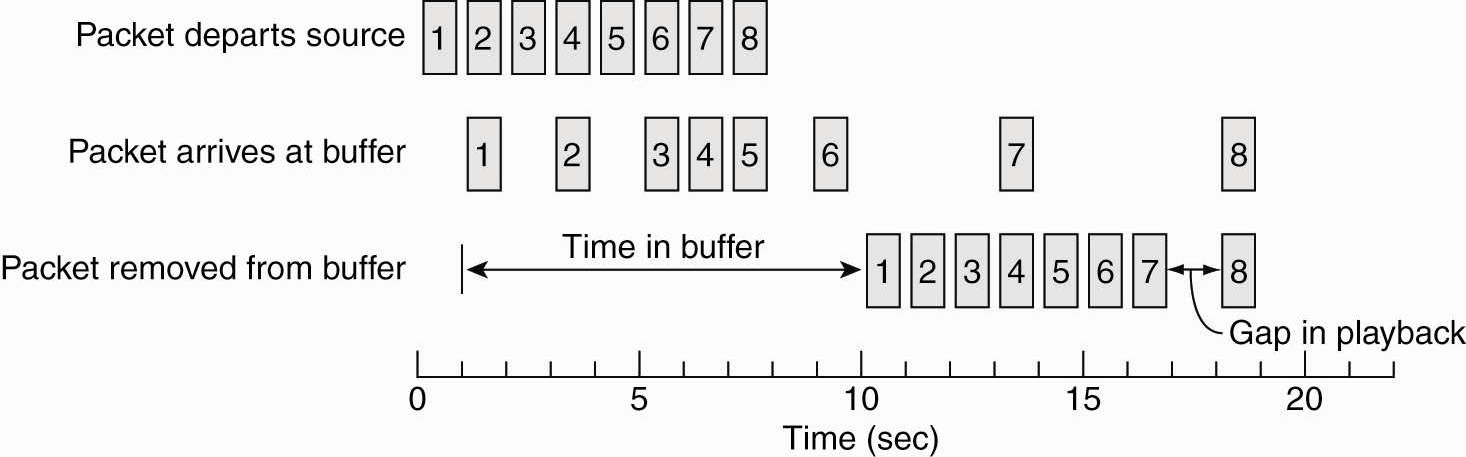
\includegraphics[scale=0.35]{img/buffer.png}
\caption{Esempio di utilizzo del buffer}\label{img:buffer}
\end{figure}
Un altro problema da affronta è la perdita di pacchetti, in quanto è inammissibile richiedere il rinvio dei pacchetti al mittente; è quindi necessario applicare delle tecniche di correzione degli errori. Una tecnica è quella di codificare i pacchetti in modo tale che qualsiasi $k$ pacchetti persi tra gli $n$ ricevuti siano sufficienti per ricostruire $k$ pacchetti corretti. Un altro problema è quando un pacchetto contiene molti frame audio e video, in questo caso l'utente può percepire un notevole vuoto nella riproduzione. Tale vuoto può essere aggirato dall'uso di frame \emph{interleaving} come mostrato nella \figurename\,\ref{img:interleaving} in questo modo il vuoto viene distribuito su più frame e si nota meno; questo meccanismo tuttavia richiede un buffer più grande.
\begin{figure}
\centering
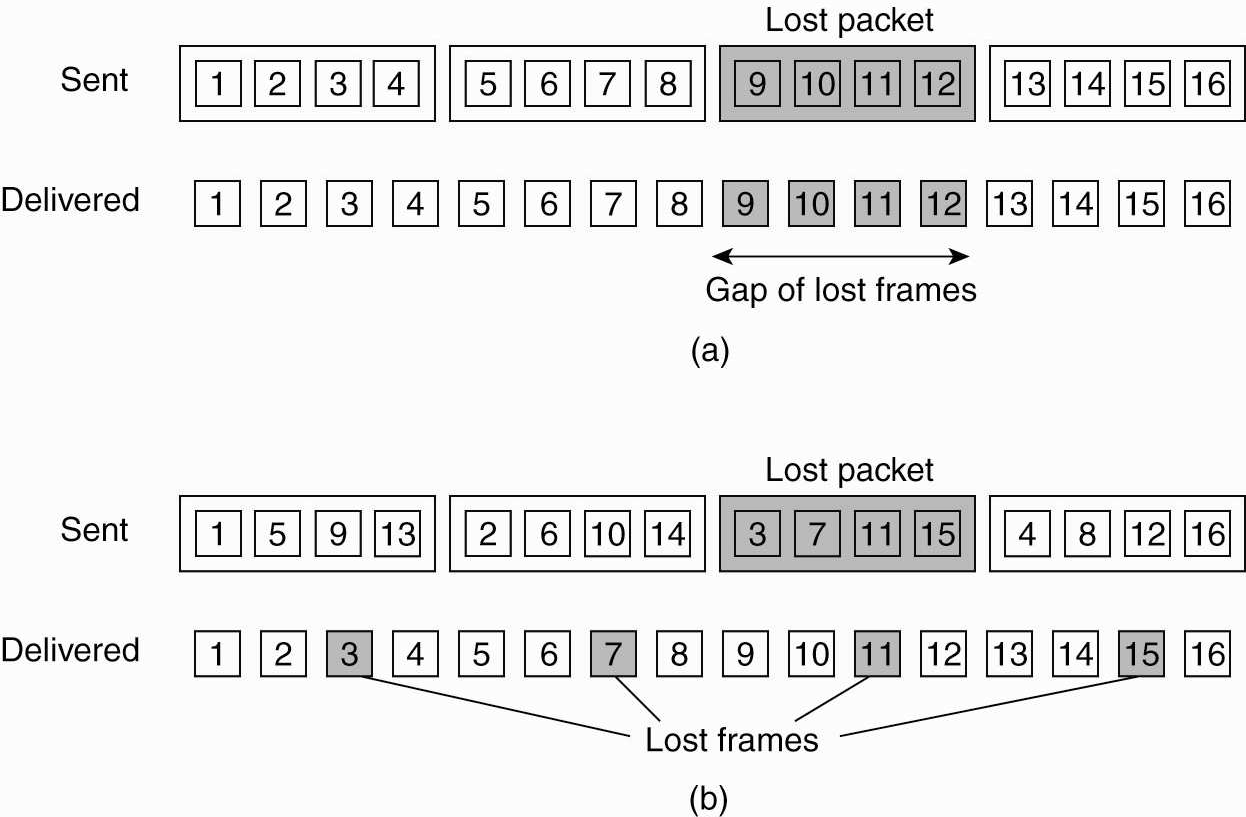
\includegraphics[scale=0.3]{img/interleaving.png}
\caption{Applicazione del meccanismo di interleaving}\label{img:interleaving}
\end{figure}
\subsubsection{Sincronizzazione degli stream}
Un elemento essenziale dei sistemi multimediali è che diversi stream eventualmente sotto forma di stream complesso, sono sincronizzati l'uno con l'altro. Sincronizzare più stream significa rispettare alcuni vincoli temporali tra gli stream.\\
Esistono diversi problemi di sincronizzazione come ad esempio la sincronizzazione di stream audio e video in un film il quale prende il nome di \emph{lip synchronization}, un altro è il problema di sincronizzare i due substream che compongono uno stream per l'audio stereo.\\
La sincronizzazione avviene a livello delle unità di dati di cui è fatto uno stream. In altre parole possiamo sincronizzare due stream solo tra unità di dati. La scelta di che cosa sia un'unità di dati dipende molto dal livello di astrazione a cui è visto lo stream.
Consideriamo uno stream audio di un CD; tale stream appare come una sequenza di campioni a 16bit con una frequenza di 44.1 kHz, la sincronizzazione con altri stream audio potrebbe avvenire ogni $23\mu sec$
\paragraph{Meccanismi di sincronizzazione}
Prima di parlare di come sincronizzare due stream dobbiamo innanzitutto distinguere i meccanismi di base per la sincronizzazione di due stream dalla distribuzione di questi meccanismi in rete.\\
Come per la granularità sulle unità di dati anche i meccanismi di sincronizzazione possono lavora a diversi livelli di astrazione. A livello più basso la sincronizzazione viene fatta sulle unità di dati. In sostanza c'è un processo che esegue semplicemente delle operazioni di lettura e scrittura su molti stream assicurandosi che queste operazioni rispettino i determinati vincoli temporali. L'inconveniente di questo tipo di sincronizzazione è che l'applicazione è completamente responsabile dell'implementazione della sincronizzazione. Un approccio migliore è quello di fornire all'applicazione un'interfaccia che le consenta di controllare più facilmente lo stream come mostrato in \figurename\,\ref{img:sincrostream}. Nei sistemi middleware per i media offrono una serie di interfacce per il controllo degli stream audio e video. Ogni dispositivo e ogni stream possiedono la loro interfaccia di alto livello inclusa quella per la notifica a un'applicazione di un cero evento.\\
Un altro aspetto da considerare è la distribuzione dei meccanismi di sincronizzazione. Nel caso sia il ricevente a dover sincronizzare uno stream complesso costituito da diversi substream esso deve sapere esattamente come procedere; in altre parole deve avere una \emph{specifica della sincronizzazione} completa e disponibile localmente. In realtà le informazioni sulla sincronizzazione vengono fornite implicitamente inviando in \emph{multiplexer} i diversi substream in un unico stream.
\begin{figure}
\centering
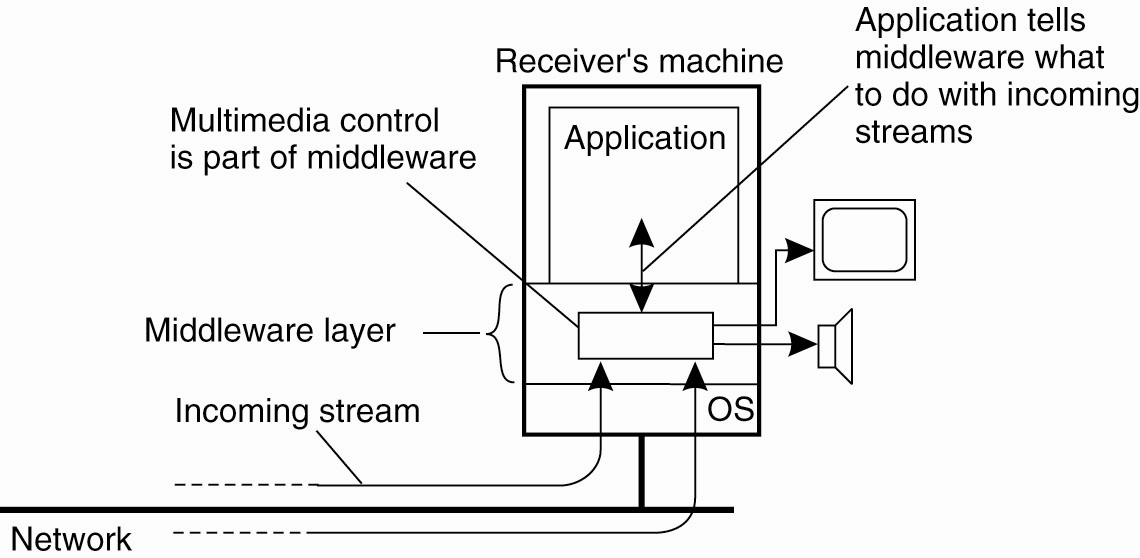
\includegraphics[scale=0.35]{img/sincrostream.png}
\caption{Sincronizzazione degli stream tramite interfacce}\label{img:sincrostream}
\end{figure}
